%%%%%%%%%%%%%%%%%%%%%%%%%%%%%%%%%%%%%%%%%%%%%%%%%%%%%%%%%%%%%%%%%%%%%%%%%%%%%%%%%%%%%%%%%
% This is a LaTeX template for Bachelor or Master theses at ZHAW, in accordance with the 
% guidelines provided here:
% https://www.zhaw.ch/en/lsfm/study/studiweb/master-ls/masters-thesis/
%
%
% This template is based on previous works by:
% Steve Gunn (http://users.ecs.soton.ac.uk/srg/softwaretools/document/templates/)
% Sunil Patel (http://www.sunilpatel.co.uk/thesis-template/)
% Matteo Delucchi (https://github.com/matteodelucchi/ZHAW_thesis-template)
%
% University specific changes were made by:
% Matteo Delucchi
% Norman Juchler
% 
% Template license:
% CC BY-NC-SA 3.0 (http://creativecommons.org/licenses/by-nc-sa/3.0/)
%%%%%%%%%%%%%%%%%%%%%%%%%%%%%%%%%%%%%%%%%%%%%%%%%%%%%%%%%%%%%%%%%%%%%%%%%%%%%%%%%%%%%%%%%

%----------------------------------------------------------------------------------------
% DOCUMENT SPECIFICATION
%----------------------------------------------------------------------------------------
\documentclass[
    11pt,                      % Default font size
    %oneside,                  % One-side binding. Default: Two-side binding / alternating margins
    english,                   % Language. Use ngerman for German (Neue Rechtschreibung)
    singlespacing,             % Spacing option: singlespacing, onehalfspacing or doublespacing
    %nolistspacing,            % Set spacing in lists to single
    %draft,                    % Enable draft mode: no pictures, no links, overfull hboxes indicated
    liststotoc,               % Include list of figures/tables/etc in the table of contents
    %toctotoc,                 % Include the main table of contents to the table of contents
    parskip,                  % Add vertical space between paragraphs
    %nohyperref,               % Disable links in the entire document
    headsepline,               % Show a horizontal line under the header
    %chapterinoneline,         % Place the chapter title and chapter number on one line
    consistentlayout,          % Have the same layout for special chapters: 
                               % declaration, abstract and acknowledgements
]{MastersDoctoralThesis}

% Uncomment the following lines to only include a subset of chapters.
% This is useful for long documents, as typesetting takes a bit of time
%\includeonly{
%    Front/titlepage,
%    Front/imprint,
%    Front/abstract,
%    %Front/declaration,
%    %Front/acknowledgements,
%    %Front/symbols,
%    Chapters/Chapter1,
%    %Chapters/Chapter2
%    }


%----------------------------------------------------------------------------------------
% PREAMBLE: PACKAGES AND CONFIGURATIONS
%----------------------------------------------------------------------------------------
% !TEX root = main.tex

%----------------------------
%   Fonts and characters
%----------------------------

% Support for special characters
\usepackage[utf8]{inputenc}    % Specify input encoding
\usepackage[T1]{fontenc}       % Specify font encoding

% Set main fonts
% Fonts catalogue: https://tug.org/FontCatalogue/
\usepackage{mathpazo}          % Use the Palatino font by default
\usepackage{beramono}          % Override the monospace/typewriter font

% ZHAW title font
% Try to load Helvetica Rounded Bold, and OpenType font.
% Loading OTF or system fonts is possible with XeLaTeX.
% If the document is compiled using pdfLaTeX, resort 
\usepackage{ifxetex}
\ifxetex
    \usepackage{fontspec}
    \newfontfamily\zhawtitlefont{Helvetica Rounded Bold}
\else
    \newcommand{\zhawtitlefont}{\scshape}
\fi

%\usepackage[scaled]{helvet}

%----------------------------
%   Environments
%----------------------------

\usepackage{caption}           % Customized caption
\usepackage{subcaption}        % Subfigure captions
\usepackage{makecell}          % Per-cell formatting in tables (\makecell)
\usepackage{pdfpages}          % Required to include PDF files/graphics (\includepdf)

\usepackage{todonotes}         % Introduces the command \todo
\setlength{\marginparwidth}{2.5cm} % Adjust this if the todo notes are out of margins

% Create boxes as follows:
% \begin{colorbox}{red}{2}
\usepackage{tcolorbox}
\newtcolorbox{textbox}[2]{
    arc=3pt,
    boxrule=#2pt,
    colback=#1!25!white,
    width=\textwidth,
    halign=left,
    valign=center,
    colframe=#1!75!black
}

%----------------------------
%   Colors
%----------------------------

% Set up colors
\usepackage{xcolor}
% ZHAW Blue: Pantone 2945 U / R0 G100 B166
\definecolor{zhawblue}{rgb}{0.00, 0.39, 0.65}
% Colors related to code listings
\definecolor{codegreen}{rgb}{0,0.6,0}
\definecolor{codegray}{rgb}{0.5,0.5,0.5}
\definecolor{codepurple}{rgb}{0.58,0,0.82}
\definecolor{codebackground}{rgb}{0.93,0.94,0.95}

%----------------------------
%   Code listings
%----------------------------

% Setup code listings
\usepackage{listings}
\lstdefinestyle{mystyle}{
    backgroundcolor=\color{codebackground},   
    commentstyle=\color{codegreen},
    keywordstyle=\color{magenta},
    numberstyle=\tiny\color{codegray},
    stringstyle=\color{codepurple},
    basicstyle=\ttfamily\footnotesize,
    breakatwhitespace=false,
    breaklines=true,
    captionpos=b,
    keepspaces=true,
    numbers=left,
    numbersep=5pt,
    showspaces=false,
    showstringspaces=false,
    showtabs=false,
    tabsize=4
}
\lstset{style=mystyle}

% minted is an alternative code listing package. (See chapter 2)
% For it to run successfully, ensure the following:
% - the Python package Pygments. Install with the following command:
%       python -m pip install Pygments
% - pdflatex (or xelatex) is executed with the flag --shell-escape
%   If you are using a TEX editor, you can modify the typesetting 
%   command somewhere in the settings.
%\usepackage[outputdir=build]{minted}
%\usemintedstyle{xcode}
% For fancier coloring schemes, see here:
% https://tex.stackexchange.com/questions/585582
% One could also create an own style in Pygments
% https://pygments.org/docs/styles/#creating-own-styles

%----------------------------
%   References
%----------------------------

% Set up references
\usepackage[
    backend=biber,             % Use biber backend (an external tool)
    %sorting=none,              % Enumerates the reference in order of their appearance
    %style=numeric-comp         % Choose here your preferred citation style, for APA choose style=apa
    style=apa
    ]{biblatex}

\usepackage[autostyle=true]{csquotes} 
                               % Required to generate language-dependent quotes 
                               % in the bibliography

%----------------------------------------------------------------------------------------
%   MARGIN SETTINGS
%----------------------------------------------------------------------------------------

\geometry{
    paper=a4paper,      % Change to letterpaper for US letter
    inner=2.5cm,        % Inner margin
    outer=3.8cm,        % Outer margin
    top=1.5cm,          % Top margin
    bottom=1.5cm,       % Bottom margin
    bindingoffset=.5cm, % Binding offset
    %showframe,         % Show the type block of the page
}
\setlength{\parskip}{1em}
\usepackage{enumitem}          % Layout control for list environments (e.g, itemize)
%\setlist{noitemsep}           % Suppress extra spaces between items
%\setlist{nosep}               % Suppress spaces before/after list environments

\addbibresource{Bibliothek.bib}
\addbibresource{Farmbot.bib}


%----------------------------------------------------------------------------------------
% THESIS INFORMATION: MODIFY THIS SECTION!
%----------------------------------------------------------------------------------------

% The information below is used in the following parts:
% - Title page
% - Imprint
% - Abstract / Zusammenfassung
% - Meta information of PDF

\thesistitle{Digital Twin for Autonomous Robots using ROS2}             % Thesis title,              command: \ttitle
\thesistype{Project Work 2}             % Type of thesis (e.g. Master Thesis) \ttype
\thesisdate{\today}                     % Date of submission                  \tdate
\keywords{robotics, gazebo, rviz, ubuntu, linux, ros2 rolling, digital twin,AMRs, URDF, SDF, Robot State Publisher }
                                        % Keywords for the thesis,            \keywordnames
\author{Noirin Graham}                  % Your name,                          \authorname
\degree{Bachelor of Science}          % Degree name,                        \degreename
\studyprogram{Applied Digital Life Sciences, B.Sc.} 
                                        % Study program                       \studyprog
\studyprogramlink{https://www.zhaw.ch/en/lsfm/studies/bachelor/applied-digital-life-sciences/}
                                        % Link to study program               \studyproglink

\supervisorA{Dr. Christian Glahn}       % Name of supervisor 1,               \supnameA
\supervisorAmail{glah@zhaw.ch}         % Email address of supervisor 1,      \supmailA
\supervisorAweb{https://www.zhaw.ch/en/about-us/person/glah/}  %            \supwebA
\supervisorAinfo{                       % Formatted info about supervisor 1:  \supinfoA
    \supnameA\\
    Zurich University of Applied Sciences\\
    Email: \href{mailto:\supmailA}{\supmailA}\\
    Web: \href{\supwebA}{Link}
}

% Keep empty if there is no supervisor 2: \supervisorB{}
\supervisorB{Christoph Koller}              % Name of supervisor 2,               \supnameB
\supervisorBmail{kolc@zhaw.ch}       % Email address of supervisor 2,      \supmailB
\supervisorBweb{https://www.zhaw.ch/en/about-us/person/kolc/}                  % \supwebB
\supervisorBinfo{                       % Formatted info about supervisor 2:  \supinfoB
    \supnameB\\
    Zurich University of Applied Sciences\\
    Email: \href{mailto:\supmailB}{\supmailB}\\
    Web: \href{\supwebB}{Link}
}

\university{Zurich University of Applied Sciences}
                                        % University name                     \univname
\universitygerman{Zürcher Hochschule für Angewandte Wissenschaften}
                                        % University, in German               \univnameger
\department{Life Sciences and Facility Management} 
                                        % Department,                         \deptname
\institute{Institute of Computational Life Sciences} 
                                        % Institute,                          \instname
\group{Center of Computational Health} 
                                        % Research group                      \groupname

% Links
\universitylink      {https://www.zhaw.ch/en/university/}                   % \univlink
\universitylinkgerman{https://www.zhaw.ch/de/hochschule/}                   % \univlinkger
\departmentlink      {https://www.zhaw.ch/en/lsfm/}                         % \deptlink
\institutelink       {https://www.zhaw.ch/en/lsfm/institutes-centres/icls/} % \instlink
\grouplink           {https://www.zhaw.ch/en/lsfm/institutes-centres/icls/computational-health/} % \grplink



\AtBeginDocument{
\hypersetup{pdftitle=\ttitle} % Set the PDF's title to your title
\hypersetup{pdfauthor=\authorname} % Set the PDF's author to your name
\hypersetup{pdfkeywords=\keywordnames} % Set the PDF's keywords to your keywords
}
\begin{document}

% \frontmatter                  % Roman page numbering for the pre-content pages
% \pagestyle{plain}             % Default to the plain heading style until the thesis style 
%                               % is called for the body content


%----------------------------------------------------------------------------------------
% TITLE PAGE AND IMPRINT
%----------------------------------------------------------------------------------------
% !TEX root = ../main.tex

%----------------------------------------------------------------------------------------
% TITLE PAGE
%----------------------------------------------------------------------------------------

\newgeometry{margin=1in}
\begin{titlepage}

% Make the title page mostly inert to the parskip-setting.
\setlength{\parskip}{0pt}

\begin{center}

\includegraphics[width=0.15\textwidth]{Figures/zhaw_rgb}

\ifxetex
    \vspace{0.6cm}
    {\zhawtitlefont\color{zhawblue}\LARGE \univname\par}   % University
    \vspace{0.2cm}
\else
    \vspace{0.87cm}
    {
\includegraphics[height=17.9pt]{Figures/zhaw_font_eng_font}\par}
    \vspace{0.05cm}
\fi
{\Large Department \deptname\par}                      % Department
\vspace{0.2cm}
{\Large \instname\par}                                 % Institute
\vspace{3.5cm}                            
\textsc{\Large \ttype}                                 % Thesis type
\vspace{0.2cm}
\HRule 
\vspace{0.4cm}
{\huge \bfseries \ttitle\par}                          % Thesis title
\vspace{0.4cm}  
\HRule
\vspace{1.5cm}

 
\begin{minipage}[t]{0.4\textwidth}
\begin{flushleft} 
    \large
    \emph{Author:}\\
    \authorname
\end{flushleft}
\end{minipage}
\begin{minipage}[t]{0.4\textwidth}
\begin{flushright} 
    \large
    \emph{Supervisors:} \\
    \supnameA \\
    \supnameB
\end{flushright}
\end{minipage}
\vspace{2cm}
 
\vfill

{\large
Submitted on\\
\tdate\\
\vspace{1.5cm}
Study program:\\
\studyprog\\
}
\vfill
\end{center}
\end{titlepage}
\restoregeometry

\let\cleardoublepage\clearpage
\pagenumbering{gobble}
% !TEX root = ../main.tex

%----------------------------------------------------------------------------------------
% IMPRINT
%----------------------------------------------------------------------------------------

\thispagestyle{empty}
\vspace*{\fill}

{\bfseries  \Large Imprint}
\vspace{0.75cm}

\begin{footnotesize}


\begin{flushleft} 
\begin{tabular}{ @{}lp{0.6\textwidth}@{} } 
\emph{Project:}  & \ttype\\ 
\emph{Title}:    & \ttitle\\
\emph{Author}:   & \authorname\\
\emph{Date}:     & \tdate\\
\emph{Keywords}: & \keywordnames\\
\emph{Copyright}:& \univname

\end{tabular}
\end{flushleft}

\vspace{0.75cm}


\begin{minipage}[t]{0.95\textwidth}
\begin{flushleft} 
\emph{Study program:}\\
\href{\studyproglink}{\studyprog}\\
\href{\univlink}{\univname}
\end{flushleft}
\end{minipage}

\vspace{0.75cm}

\begin{minipage}[t]{0.50\textwidth}
\begin{flushleft} 
\emph{Supervisor 1:}\\
\supinfoA
\end{flushleft}
\end{minipage}
\begin{minipage}[t]{0.45\textwidth}
\begin{flushleft} 
\ifdefempty{\supnameB}
{}
{
    \emph{Supervisor 2:}\\
    \supinfoB
}
\end{flushleft}
\end{minipage}

\end{footnotesize}



%----------------------------------------------------------------------------------------
% DECLARATION
%----------------------------------------------------------------------------------------
% Comment out this section if the declaration of originality from ZHAW is used.
% !TEX root = ../main.tex

%----------------------------------------------------------------------------------------
% DECLARATION OF ORIGINALITY
%----------------------------------------------------------------------------------------

\begin{declaration}
\addchaptertocentry{\authorshipname} % Add the declaration to the table of contents

\begin{textbox}{red}{2}
REMOVE THIS SECTION IF THE \href{https://www.zhaw.ch/en/lsfm/study/studiweb/master-ls/masters-thesis/}{ORIGINAL COPY OF THE ZHAW DECLARATION OF ORIGINALITY} IS USED IN THE APPENDIX.
\end{textbox}
\vspace{1cm}

\noindent I, \authorname, declare that this thesis titled, \enquote{\ttitle} and the work presented in it are my own. I confirm that:

\begin{itemize} 
\item This work was done wholly or mainly while in candidature for a research degree at the \univname.
\item Where any part of this thesis has previously been submitted for a degree or any other qualification at this university or any other institution, this has been clearly stated.
\item Where I have consulted the published work of others, this is always clearly attributed.
\item Where I have quoted from the work of others, the source is always given. With the exception of such quotations, this thesis is entirely my own work.
\item I have acknowledged all main sources of help.
\item Where the thesis is based on work done by myself jointly with others, I have made clear exactly what was done by others and what I have contributed myself.\\
\end{itemize}
\vspace{1cm}

\noindent Signed:\\
\rule[0.5em]{25em}{0.5pt} % This prints a line for the signature
 
\noindent Date:\\
\rule[0.5em]{25em}{0.5pt} % This prints a line to write the date
\end{declaration}

\cleardoublepage

%----------------------------------------------------------------------------------------
% ABSTRACT
%----------------------------------------------------------------------------------------
% !TEX root = ../main.tex

%----------------------------------------------------------------------------------------
% ABSTRACT PAGE
%----------------------------------------------------------------------------------------
\begin{abstract}
\addchaptertocentry{\abstractname} % Add the abstract to the table of contents
This project presents the development of a simplified digital twin of an autonomous robot. The three\-wheeled robot was recreated as a digital twin using ROS2, an advanced open-source robotics software. The project was developed in the ros2 rolling distribution. Throughout the project, the robot's description could be successfully captured in a developed URDF file, which used the marco language xacro. The URDF file could be spawned successfully in the visualization tool rviz2 as well as the simulator gazebo ionic. For the control system within the gazebo environment, the differential diver plugin was implemented. The two repositories ros\_arduino\_bridge and serial\_motor\_demo were used as a starting point for the robot control system. These repositories contained a network of ros2 nodes, which communicated motor speed over the motor\_command topic. To tailor the given nodes to the requirements of the project an additional node was developed, which communicated with the /cmd\_vel and motor\_command topics. The main goal of the project could be met, by simply finding some phases of the project. Instead of a sophisticated control system like the ros2\_conrtol and ros2\_controller packages, the native communication system relying on nodes and topics was used in the project. Further, the connection between the gazebo simulator and the rviz2 visualizer and feedback messages from the motor controller to the rviz2 visualizer could not be established. However, the synchronization of the DT and the real\-world robot movement could be established.
\end{abstract}



%----------------------------------------------------------------------------------------
% ACKNOWLEDGEMENTS
%----------------------------------------------------------------------------------------
%% !TEX root = ../main.tex

%----------------------------------------------------------------------------------------
% ACKNOWLEDGEMENTS
%----------------------------------------------------------------------------------------
\begin{acknowledgements}
\addchaptertocentry{\acknowledgementname} % Add the acknowledgements to the table of contents

The acknowledgements belong here. Do not forget to mention your project supervisors, without flattering them too much.
\end{acknowledgements}



%----------------------------------------------------------------------------------------
% LIST OF CONTENTS/FIGURES/TABLES PAGES
%----------------------------------------------------------------------------------------
% Comment out if any of the following is not needed:
\tableofcontents  % Add main table of contents
\listoffigures    % Add list of figures
%\listoftables     % Add list of tables

%----------------------------------------------------------------------------------------
% START ENUMERATING (ARABIC) 
%----------------------------------------------------------------------------------------
% \cleardoublepage
% \pagenumbering{arabic}  
% \setcounter{page}{1} 
% \mainmatter
% \pagestyle{plain}        % Seitenzahlen in der Fußzeile

%----------------------------------------------------------------------------------------
% ABBREVIATIONS / SYMBOLS
%----------------------------------------------------------------------------------------
% !TEX root = ../main.tex

%----------------------------------------------------------------------------------------
% ABBREVIATIONS
%----------------------------------------------------------------------------------------

% List of abbreviations: a table of two columns.
\begin{abbreviations}{ll}

    \textbf{ROS2} & \textbf{R}obot \textbf{O}perating \textbf{S}ystem \textbf{2}\\
    \textbf{RViz2} & \textbf{R}OS \textbf{V}isualization tool version \textbf{2}\\
    \textbf{Gazebo} & Simulation tool for robotics\\
    \textbf{DT} & \textbf{D}igital \textbf{T}win\\
    \textbf{URDF} & \textbf{U}nified \textbf{R}obot \textbf{D}escription \textbf{F}ormat\\
    \textbf{Xacro} & \textbf{X}ML \textbf{Macro}\\
    \textbf{SDF} & \textbf{S}imulation \textbf{D}escription \textbf{F}ormat\\
    \textbf{AMR} & \textbf{A}utonomous \textbf{M}obile \textbf{R}obot\\
    \textbf{NIST} & \textbf{N}ational \textbf{I}nstitute of \textbf{S}tandards and \textbf{T}echnology\\
    \textbf{PWM} & \textbf{P}ulse \textbf{W}idth \textbf{M}odulation\\
    \textbf{LTS} & \textbf{L}ong-\textbf{T}erm \textbf{S}upport\\
    \textbf{TF} & \textbf{T}ransform (in ROS for coordinate transformations)\\
    \textbf{tf2} & ROS \textbf{T}ransform library version \textbf{2}\\
    \textbf{Odom} & \textbf{O}dometry (for estimating position and velocity)\\
    \textbf{ROS\_DOMAIN\_ID} & ROS domain configuration parameter\\
    \textbf{ROS\_IP} & IP address configuration in ROS\\
    \textbf{cmd\_vel} & \textbf{C}ommand \textbf{Vel}ocity (topic in ROS for movement control)\\
    \textbf{gz\_ros\_bridge} & \textbf{G}azebo-\textbf{R}OS \textbf{bridge}\\
    \textbf{Colcon} & Build tool for ROS2 workspaces\\
    \textbf{CMake} & Cross-platform build system\\
    \textbf{XML} & \textbf{E}xtensible \textbf{M}arkup \textbf{L}anguage\\
    \textbf{YAML} & \textbf{YAML} Ain’t \textbf{M}arkup \textbf{L}anguage (used for configuration files)\\
    \textbf{Raspberry Pi} & Single-board computer used as an onboard device\\
    \textbf{Arduino} & Microcontroller board\\
    \textbf{SSH} & \textbf{S}ecure \textbf{Sh}ell (for secure remote communication)\\
    \textbf{IDE} & \textbf{I}ntegrated \textbf{D}evelopment \textbf{E}nvironment\\
    \textbf{WSL2} & \textbf{W}indows \textbf{S}ubsystem for \textbf{L}inux \textbf{2}\\
    \textbf{VirtualBox} & Virtualization software for running virtual machines\\
    \textbf{Docker} & Platform for containerized applications\\
    \textbf{Differential Drive Plugin} & Gazebo plugin for differential drive robot control\\
    \textbf{Rolling Distribution} & Development release of ROS2 with latest features\\
    \textbf{Jazzy Jalisco} & Latest LTS distribution of ROS2\\
    \textbf{Harmonic/Ionic} & Gazebo distribution names\\
    \textbf{Motor Driver} & Interface converting control signals for motor operation\\
    \textbf{Motor Controller} & Device managing motor speeds and directions\\
    \textbf{Robot State Publisher} & ROS node for publishing robot states\\
    \textbf{Joint State Publisher} & ROS node for publishing joint states\\
    \textbf{TF Tree} & Hierarchical structure of coordinate transformations in ROS\\
    \textbf{ROS Node} & Independent computing process in ROS\\
    \textbf{ROS Topic} & Communication channel for ROS messages\\
    \textbf{Rolling Ridley} & Developer release version of ROS2 distribution\\
    
    \end{abbreviations}
    

%----------------------------------------------------------------------------------------
% PHYSICAL CONSTANTS/OTHER DEFINITIONS
%----------------------------------------------------------------------------------------

%% List of physical constants: a three column table
%\begin{constants}{lr@{${}={}$}l} 
%
%% The \SI{}{} command is provided by the siunitx package, see its documentation 
%% for instructions on how to use it
%
%Speed of Light & $c_{0}$ & \SI{2.99792458e8}{\meter\per\second} (exact)\\
%%Constant Name & $Symbol$ & $Constant Value$ with units\\
%
%\end{constants}


%----------------------------------------------------------------------------------------
% SYMBOLS
%----------------------------------------------------------------------------------------

%% List of Symbols: a three column table
%\begin{symbols}{lll} 
%
%$a$ & distance & \si{\meter} \\
%$P$ & power & \si{\watt} (\si{\joule\per\second}) \\
%%Symbol & Name & Unit \\
%
%\addlinespace % Gap to separate the Roman symbols from the Greek
%
%$\omega$ & angular frequency & \si{\radian} \\
%
%\end{symbols}



%----------------------------------------------------------------------------------------
% DEDICATION
%----------------------------------------------------------------------------------------
%\dedicatory{For/Dedicated to/To my\ldots} 
 \clearpage
 \pagenumbering{arabic}


%----------------------------------------------------------------------------------------
% THESIS CONTENT - CHAPTERS
%----------------------------------------------------------------------------------------
% \mainmatter % Begin numeric (1,2,3...) page numbering
% \pagestyle{thesis} % Return the page headers back to the "thesis" style

% Include the chapters of the thesis as separate files from the Chapters folder
% Uncomment the lines as you write the chapters

% Chapter 1: Introduction
\chapter{Introduction}

As urbanization continues to expand, integrating sustainable green spaces into densely populated areas has become a growing challenge. Rooftop solar panels, already serving as key assets in renewable energy production, present an opportunity to co\-function as natural green spaces, contributing to urban biodiversity and improved air quality. 
However, maintaining vegetation in these environments is an exhausting task, as overgrown plants can cast shadows on photovoltaic panels, reducing their efficiency but the human interference within the green spaces preferentially is kept to a minimum. 

To address this an autonomous robot capable of maintaining rooftop vegetation will be developed. The robot will be equipped with advanced decision-making capabilities to identify and trim specific plants without hindering the photovoltaic panels performance. To ensure optimal functionality and provide real-time monitoring, a digital twin will be developed to simulate, control, and oversee the robot's actions. This innovative solution combines robotics, artificial intelligence, and digital simulation to create a sustainable coexistence between green infrastructure and renewable energy technology. 

Controlling robots is complex and requires a lot of knowledge and experience, among the systems that reduce the complexity of controlling robots is the Robot Operating System (ROS2). 
Therefore, as a starting point, this project aims to learn and understand ROS2 and its applications in a concrete robotic application. Therefore, a simplified version of the envisioned autonomous robot will be used in this project.

\section{Project aim}

Within the ROS2 ecosystem, a digital twin will be developed, focusing on a control system managing the DT and the robot.
 ROS2 defines the components, interfaces and tools for building advanced robots. A robot is built out of three primary elements: actuators, sensors, and a control system. Actuators enable the robot to perform movements, sensors allow it to perceive its environment, and the control system functions as the robot's brain, processing inputs and coordinating actions.
ROS2 enables users to build these components and create a connection between them using ROS2 tools, which are called topics and messages. The visualization and simulation environment, such as rviz2 and gazebo, provides powerful tools for developing and testing robotic systems in a virtual space before deploying them in the real world \autocite{openroboticsROSHome}.





% Chapter 2: Literature Review
\chapter{Literature Review}

This literature review examines the background and relevant technologies that form the foundation for the project, focusing on ROS2, its components, and the role of digital twins in robotic applications. 

\section{Digital Twin}
Digital Twin (DT) technology is an emerging field that continues to expand rapidly. Although many industries have begun adopting this technology, the definition of a Digital Twin remains ambiguous in the literature. Some authors define it as a virtual representation of a physical system, while others emphasize the exchange of information between two domains, incorporating sensors, data, and models \autocite{staczekDigitalTwinApproach2021}. In this report, the definition provided by the National Institute of Standards and Technology (NIST) will be used:

\begin{quote}
``A digital twin is the electronic representation—the digital representation—of a real-world entity, concept, or notion, either physical or perceived \autocite{voasDraftConsiderationsDigital2021}.''
\end{quote}

A DT functions as a model or simulation that offers static or dynamic views of its real-world counterpart. It integrates modeling, simulation, and real-time data to replicate the behaviour of its physical counterpart. Unlike static models, DTs are continuously updated in real-time.
The distinction between a DT and a mirroring system often overlaps, making it challenging to define a clear boundary. In this project, a digital twin is defined as a electronic representation of its real-world counterpart, capturing its electrical and functional characteristics. While both components can be controlled simultaneously, their behaviors remain distinct and unique to each system. Conversely, a mirroring system involves two counterparts that move synchronously, with the motion dictated either by the virtual model or the real-world robot.
DTs are applicable in various domains, such as simulating behaviour over time (Dynamic Modeling) or controlling physical systems through bidirectional communication, such as managing unmanned aerial vehicles (UAVs) or autonomous mobile robots (AMRs).
However, this technology introduces several challenges, including cybersecurity risks, heightened complexity, and ensuring the accuracy of the digital twin representation \autocite{voasDraftConsiderationsDigital2021}.


\section{Autonomous Robots}

An autonomous robot is defined as a system that can handle various environmental constraints automatically while completing a task. It is equipped with the necessary methods to adjust to its surroundings without requiring constant human input \autocite{wahdeINTRODUCTIONAUTONOMOUSROBOTS2016}. 
The predecessors of autonomous robots are conventional robots that are widely used in manufacturing across various industries for over two decades. Conventional robots operate by executing preprogrammed instructions or direct commands.
Autonomous robots are designed to increase flexibility and adaptability. These advanced systems can adapt to environmental constraints and perform tasks with minimal human intervention. 
A notable subclass of autonomous robots is mobile robots \autocite{fahimiAutonomousRobotsModeling2009}. 
In this project, the focus will lay on developing a digital twin of an autonomous mobile robot (AMR). AMRs, the latest advancement in unmanned mobile robots, are predominantly used in large warehouses for material handling. These robots are designed to move across a defined area and navigate through an environment to perform a specific task, while human intervention is kept at a minimum. Decisions on where and when to act are based on predefined programming and environmental inputs. 
In order to develop an AMR that is able to perform tasks autonomously a DT is essential. The open-source software ros2 offers a variety of a highly functional tool, which simplifies the process of building a DT significantly \autocite{staczekDigitalTwinApproach2021}.


%% CG: The entire ROS section should be placed in a separate chapter on the ROS2 architecture and concepts. After reading this part I would even consider it to be part of the method section.

\section{What is ROS?}

The robot operating system is an advanced open-source robotics software that provides a collection of software libraries and tools to help developers build robot software, offering features such as hardware abstraction, device drivers, libraries for commonly used algorithms, and message-passing between processes. 
The first version of ROS had a significant role in the maturing robot industry, the ROS ecosystem has become influential in nearly every intelligent machine sector.
The successor ROS2 was developed to address the limitations such as lack of security, low reliability in non-ideal environments and limited real-time support of its predecessor. The architecture of ROS2 is divided into three categories Middleware, Algorithms and Developer tools \autocite{macenskiRobotOperatingSystem2022}.

\subsection{What is a ROS distribution}

A distribution contains a collection of interrelated software components, tools, libraries and infrastructure that are bundled together and released at specific intervals. 
ROS as well as ROS2 are available in a sequence of distributions, these are essentially stable releases that include the core components which are required to build and run robotic systems. 
In the ROS ecosystem, there are two main types of distributions available: Long-Term Support (LTS) distributions and non-LTS (development) distributions. The main difference between the two lies in their update and maintenance policies.
LTS distributions are designed for stability and reliability, with updates provided at defined intervals, primarily focusing on bug fixes and security patches. The latest long-term support(LTS) distribution is the "Jazzy Jalisco", which was released on May 23rd, 2024 \autocite{openroboticsJazzyJaliscoJazzy}.

In contrast, non-LTS (development) distributions reflect the latest state of ROS development. This distribution includes the latest changes and features of ROS 2. Unlike other stable distributions, the non-LTS distribution is not focused on long-term stability but instead is constantly updated. It serves two purposes:

\begin{enumerate}
    \item It is a staging area for future stable distributions of ROS 2, and
%% CG: This is not a purpose
    \item It is a collection of the most recent development releases.
%% CG: This is a purpose ;)
    \item allows for testing existing solutions for upcoming ROS distributions.
\end{enumerate}

Due to it's frequent changes and potential instability it is not recommended for use in production environments. Within the ROS ecosystem, the rolling distribution takes on the role of the non-LTS (development) distributions \autocite{openroboticsDistributionsROS2a}.

\subsection{Nodes and Topics}

The simple explanation of a node is the following; nodes are executable files within a ROS2 package. Each node should be responsible for a single modular purpose. To send and receive data from other nodes, messages can be sent to a topic \autocite{openroboticsUnderstandingNodesROS}. A graphical overview of the interaction between nodes and topics is given in the figure~\ref{fig:Node_topics}. In order for this system to work properly the two nodes need to be accessible from the same network, further information regarding the network configuration will be discussed in the next chapter . 

\begin{figure}[h]
    \centering
    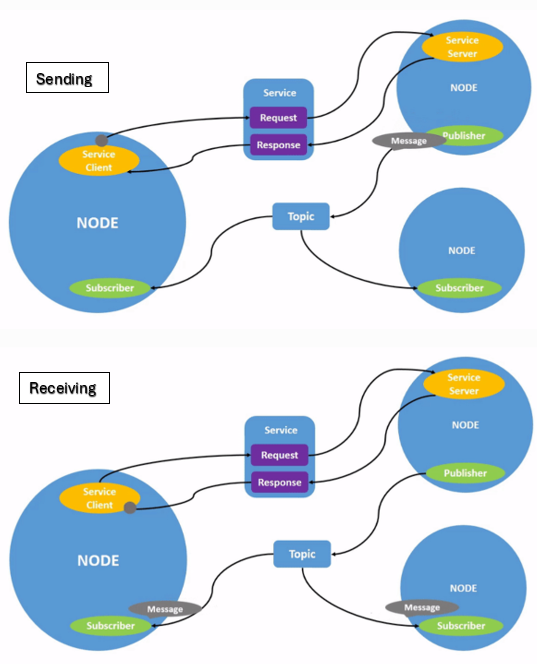
\includegraphics[width=0.7\textwidth]{Figures/Nodes_topics.png}
    \caption{URDF components relationships}
    \label{fig:Node_topics}
    \autocite{Interaction nodes and topics}
\end{figure}

\newpage
\section{Rviz and Gezebo}

ROS2 provides a variety of visualization and simulation tools, some developed within the ROS ecosystem and others designed to be compatible with it. Within the scope of this Project, the visualization tool RViz and the simulation tool Gazebo were chosen to support the development and implementation of the digital twin.

\subsection{RViz}
RViz is a ROS toolkit that enables the visualization of data and algorithms in real-world domains, including 2D and 3D spaces. It can work with various data structures, enabling its use across different computational and scientific fields. \autocite{kamRVizToolkitReal2015}

\subsection{Gazebo}

Gazebo is an open-source collection of modular software libraries aimed at simplifying the development of high-performance robotics and simulation applications.\autocite{openroboticsGazebo}

\subsection{Combination of RViz and Gazebo}

RViz itself does not provide a built-in simulation, therefore a parallel usage of Gazebo is widely used. Gazebo handles the physics-based simulation of robots and their environments, while RViz provides a real-time visual interface to display the simulation data. Together, they allow users to visualize the robot's movements, map generation, sensor data, and coordinate transformations, as well as to interact with the robot by sending commands or testing navigation and planning strategies in a controlled environment.\autocite{indriAMRSystemAutonomous}
In order to develop and implement a digital twin with the support of the two tools the robot's physical structure and configuration must be defined in a specific format.

\section{URDF, Xacro and SDF}

The Unified Robotic Description Format (URDF) is an XML file format used in ROS and ROS2 to define a robot's physical structure and configuration. It provides a 3D representation of the robot, specifying details about its joints, links, sensors, and their respective properties. This effectively describes the robot's physical design and behaviour. The diagram, as shown in Figure~\ref{fig:URDF_comp}, form the ROS wiki illustrates the relationships between these components \autocite{openroboticsUrdfROSWiki}.
URDF files are created to define the kinematic and dynamic properties of a single robot in isolation. 
To develop a more complex system, which includes sensors, actuators or a second robot most developers use the macro language xacro (XML macro). It enhances URDF files by allowing for conditional logic, variables, and parameterization, enabling developers to make these files configurable and maintainable. 
A Modular Xacro splits up the robot description into multiple separate child Xacro files, each with a specific purpose. These files are then included in a parent Xacro file. The modular structure typically includes:

\begin{enumerate}
    \item Robot Description File: Contains the main robot model description, such as links, joints, and kinematics.
    \item Material List File: Defines materials and visual properties, such as colors and textures used in the model.
    \item Configuration File: Includes parameters and settings required for simulation in tools like Gazebo, such as physical properties and plugin configurations.
\end{enumerate}

A Xacro file itself is an enhanced version of a URDF (Unified Robot Description Format) file, enriched with Xacro-specific tags to support macros, parameterization, and modular inclusion.
At runtime, the Xacro program preprocesses the parent Xacro file along with its included files to generate a standard URDF. This URDF file is then used by simulation tools (e.g., Gazebo) or visualization tools (e.g., RViz) \autocite{albergoUnderstandingXacroMisunderstandings2022}.
Another way to make URDF suitable for a gazebo simulation, without using Xacro, is to translate the URDF file to the native Simulation Description Format (SDF) of Gazbeo. The translation process includes the implementation of simulation-specific tags to the URDF file. These tags define attributes such as the robot's pose, friction, inertial elements, and other physical properties. Furthermore, these tags can describe the surroundings of the robot and thereby place the robot in a simulated world. 
Converting a URDF to SDF is straightforward and is achieved by adding Gazebo plugins to the URDF file. Essentially, Gazebo plugins create a communication interface (referred to as a Topic in ROS) between ROS and Gazebo. The control processes in ROS communicate through a Publish/Subscribe model on these Topics \autocite{takayaSimulationEnvironmentMobile2016}.

\begin{figure}[h]
    \centering
    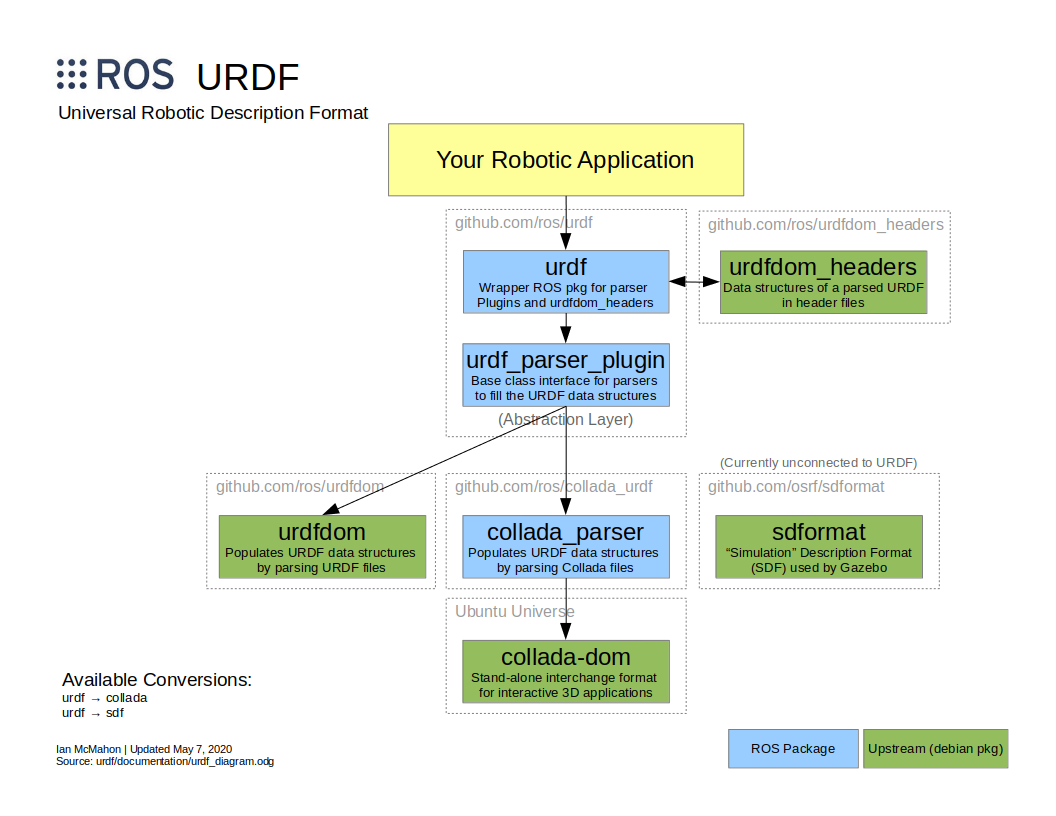
\includegraphics[width=0.7\textwidth]{Figures/urdf_diagram.png}
    \caption{URDF components relationships}
    \label{fig:URDF_comp}
\end{figure}
\autocite{openroboticsUrdfROSWiki}


% Chapter 3: Methodology
\chapter{Methods}

\section{Project Pipline}

The project pipeline contains 8 distinct phases that are shown in the figure~\ref{fig:pipline}. 
The pipeline begins by building the physical prototype of the robot. 
The second phase involved setting up the hardware and software required for the project, which included the initial introduction to the ROS 2 ecosystem. This phase involved learning and implementing foundational concepts necessary for the subsequent stages of the project. 
The third phase implements the ROS2 installations and tests its functionality by establishing a connection through two nodes, one running on the onboard computer and another on the control unit. 
The fourth phase carries out the development of the URDF file. 
The fifth phase vizualizes the URDF file in the RViz2 visualizer, and establishes the joint movement by using the package "joint state publisher." 
The sixth phase includes the simulation of the model within the Gazebo simulator. The DiffDrive plugin was used to control the simulation.
The seventh phase tested the remote control of the motor of the physical robot by using two ROS2 nodes: one listening for motor speed commands and one sending the motor speed commands. In the last phase, the three components—RViz, Gazebo, and drive node—were concatenated in a launch file and run simultaneously. 
This pipeline doesn't necessarily follow the structure of a best practice case, it shows how this project was built. 

\begin{figure}[h]
    \centering
    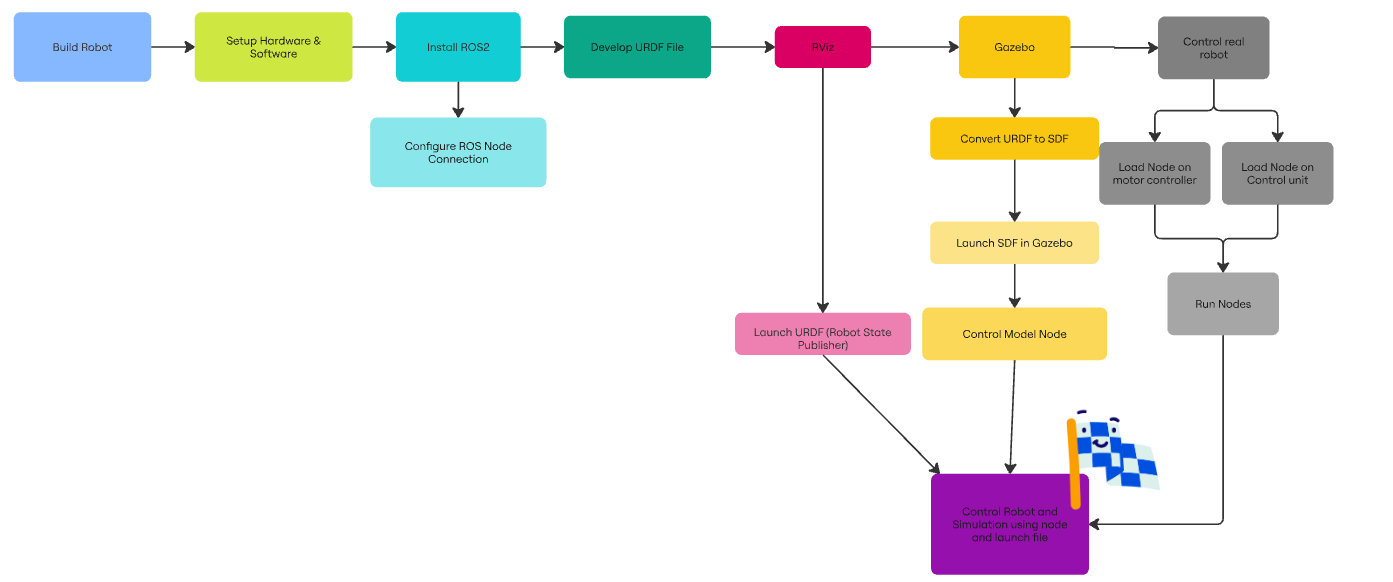
\includegraphics[width=0.9\textwidth]{Figures/project_pipline.png}
    \caption{Project Pipline}
    \label{fig:pipline}
\end{figure}
\autocite{openroboticsUrdfROSWiki}

\newpage
\section{Robot parts}

%% CG: check for repetetive phasing. 

The core elements may differ for different robot types, for this project, the core elements which were used to control the robot were the following: 

\begin{enumerate}
    \item motors
    \item power stations
    \item the motor drive
    \item the motor drive
    \item onboard computer
\end{enumerate}

The motors are the basic components which were used to give the robot the ability to move. In order to run the motors a power station which provides the appropriate voltage was included. By supplying the motors with electricity a basic movement of the motor could be achieved. 
To change the speed or direction and control them remotely, the robot was utilised with a motor driver. The motor driver took a low voltage and low current signal, primarily in the form of pulse width modulation (PWM), from the controller and amplified it using the power supply, creating a higher voltage and current feed to drive the motor.
The PWM signal consisted of a series of fast pulses, where the averaged value over time determined the percentage of the total voltage supplied to the motor. This ratio of on-time to off-time, known as the duty cycle, was implemented to regulate motor operation.
The motor control used more practical input formats, such as target speed, to calculate the appropriate signal for the driver. The driver, in turn, amplified this signal and transmitted it to the motor. A communication layer, a serial connection, was established to link the onboard computer with the motor controller. This communication allowed the onboard computer to send target speeds to the motor control.
The onboard computer was equipped with ROS2. The key tasks of ROS2 were to calculate the target motor speeds and translate these into a protocol compatible with the motor controller.

\section{System Setup of computer hardware and Software}

There are various computer hardware and software configurations available for working with ROS2, ranging from using a virtual machine with a Linux Ubuntu operation system (OS), to running a Docker container with a selected ROS2 image that can be run on a Windows OS by using the WSL2 \autocite{dockerRosOfficialImage}, or directly installing ROS2 on computer hardware that has Ubuntu Linux installed.
 In this project, all the previously mentioned methods were explored. The detailed experience will be discussed in more detail in the results in the chapter ''Installation computer hardware and software''.

\subsection{ROS2 installation}

The next step included the installation of the ROS2 Rolling on both the control unit and edge device. A detailed description of the installation can be found the installation guide A2. For Ubuntu 24.04 LTS the ROS2 distribution Rolling Ridely or Jazzy Jalisco can be used. For this stage of the project, the Rolling Ridely distribution was used. The Rolling Ridely is the rolling development distribution, which means it continuously integrates the latest features, updates and improvements \autocite{openroboticsDistributionsROS2}. This also makes it more unstable than the Jazzy Jalisco, which introduces several complications, as will be discussed in a later chapter. To guarantee a stable model in the future, a distribution change will be necessary. 

\subsection{Network configuration}

The network structure can be set up in multiple ways and should be dependent on the requirements a project has. For this project, two existing networks—home and ZHAW—were planted to be utilized. 


\subsection{ROS2 Nodes}

The development of the project relied heavily on the usage and development of Nodes and the communication system between nodes and topics. The primary used node was the demo node talker/listener, it was used to test the communication between the control unit and the edge device. These six additional nodes were used within this project: 

\begin{itemize}
    \item \verb|robot_state_publisher|: Publishes the URDF model to the /robot\_description topic for visualization and simulation.
    \item \verb|joint_state_publisher|: Publishes the robot's joint states for visualizing movements in RViz2.
    \item \verb|rviz2|: Launches RViz2 with a predefined configuration to visualize the robot's state.
    \item \verb|ros_gz_sim|: Simulates the environment and robot model based on control commands.
    \item \verb|ros_gz_bridge|: Connects ROS 2 and Gazebo to enable communication for movement commands.
    \item \verb|cmd_vel_to_motor_command|: Converts /cmd\_vel commands into motor commands for the real robot and Gazebo.
\end{itemize}

In order for these six nodes to send and receive data from each other the following topics where used:

\begin{itemize}
    \item \verb|/robot_description|: Publishes the robot's URDF model for visualization in RViz2 and simulation in Gazebo.
    \item \verb|/joint_states|: Publishes the state of the robot's joints.
    \item \verb|/cmd_vel|: Sends velocity commands (linear and angular) to control the robot's movement.
    \item \verb|/motor_command|: Simulates the environment and robot model based on control commands.
    \item \verb|ros_gz_bridge|: Transmits motor-specific commands to the real robot's motor controller.
    \item \verb|/tf|: Publishes transformations for coordinate frames.
\end{itemize}



\section{Develop URDF File}

To create a digital twin, a robot description is required. This description contains all the information about the robot's physical characteristics and is stored in a URDF file. The structure of a URDF file follows a simple and repetitive pattern. At its core, it consists of a tree of links connected by joints. The links represent the robot's physical components, such as wheels, while the joints define the dynamic relationships between these components—for example, the rotation of a wheel relative to the robot's body.
When defining a joint, a specific type must be assigned. The available joint types are:

\begin{itemize}
    \item Revolute: Rotational motion with defined minimum and maximum angle limits.
    \item Continuous: Unlimited rotational motion, such as that of a wheel.
    \item Prismatic: Linear sliding motion with specified minimum and maximum position limits.
    \item Fixed: A rigid connection where the child link is immovably attached to the parent link, often used for "convenience" links.
\end{itemize} \autocite{newansDescribingRobotsURDF}

URDF files are written in XML, with their content represented as a series of nested tags. The primary tags used in this project include were robot tag, link tags and joint tags.

\subsection{The Robot tag}

The robot tag is the root element of the robot description file, encapsulating all other elements.  It is placed immediately following the XML declaration.  It is placed immediately following the XML declaration. \autocite{UrdfXMLROS}

\lstinputlisting[caption={Robot Tag code Example}, label={lst:robot_tag}]{Code/robot_tag.xml}

\subsection{Link tags}

The link tag defines a rigid body, specifying its visual features, and collision properties. \autocite{UrdfXMLROS}

\lstinputlisting[caption={Link Tag code Example}, label={lst:robot_tag}]{Code/link_tag.xml}

\subsection{Joint tags}

The joint tags describes the kinematics and dynamics of the joint, including its savety limits. It allways stands between a child link and it's parent link.\autocite{UrdfXMLROS} 

\lstinputlisting[caption={Joint Tag Code Example}, label={lst:robot_tag}]{Code/joint_tag.xml}

Additional tags such as sensor, model state or gazebo can be implementet. In this project, the URDF was used to establish a foundational understanding of how a robot description is configured. For the final simulation in Gazebo, the URDF file was converted into an SDF file, which is compatible with Gazebo and allows the model to be launched in the simulation environment.

\section{Launch URDF in RViz}
To visualize the URDF model, the ROS 2 visualization tool Rviz was used. There are several ways to launch a URDF in Rviz, but the simplest approach is to create a ROS 2 launch file. A ROS 2 launch file allows the simultaneous configuration and execution of multiple ROS 2 nodes. These launch files can be written in Python, XML, or YAML, depending on the project requirements. \autocite{CreatingLaunchFile}
For this project, a Python launch script was created. This script starts the following nodes.

\begin{itemize}
    \item The robot state publisher node, which publishes the robot's state to the tf2 transform tree,
    \item The joint state publisher gui node, enabling interactive control to move the robot's wheels, and
    \item The Rviz node, to visualize the URDF model in the Rviz interface.
\end{itemize}

\lstinputlisting[caption={Launch file structure}, label={lst:robot_tag}]{Code/launchfile.py}

\section{Gazebo}
The Gazebo simulator was utilized in this project to simulate the robot's behaviour and interactions within a virtual environment. Unlike RViz, Gazebo is not included as a default package in the ROS 2 Rolling installation. Similar to ROS 2, Gazebo is available in multiple distributions, each corresponding to a specific ROS 2 version. For the ROS 2 Rolling distribution, the Gazebo Ionic distribution must be installed. Detailed installation steps for Gazebo in the Rolling distribution are provided in Installation Guide A3. To launch the URDF file two options are given, the primary is to use the xacro program to create the URDF file. By doing so the necessary elements for simulation, such as link inertial properties, joint dynamics, and kinematic chains are included in the URDF file. The second option is to transition the URDF to the native Simulation Description Format (SDF) of gazebo. This option is especially recommended if additional Gazebo-specific features are needed for the model.

\section{Control the robot}

%% CG: In the methods you need to outline what you have done to understand how to control the robot and its digital twin. The actual implementation is part of the results section.

As a starting point to understand how the physical robot could be controlled remotely, a tutorial from the Articubot website was followed. This does not represent a scientific approach, however, it streamlined this part of the project significantly. The following key steps were recreated based on the tutorial:

\begin{itemize}
    \item Exploring the setup components and their interactions.
    \item Establishing an SSH connection from the control unit to the onboard computer using Visual Studio Remote.
    \item Utilizing the Arduino Extension within the Visual Studio Remote environment to upload scripts to the Arduino Mega (motor controller).
    \item Transmitting data, such as motor speed, from a node running on the control unit to the appropriate topic via messages, and receiving this data on a corresponding node running on the onboard computer.
\end{itemize}

% Chapter 3: Results
\chapter{Results}


\section{Repositories for Code Management}

A GitHub organization is created to manage all repositories related to the project. Within this organization, four main repositories essential for the project were maintained:
\begin{itemize}
    \item \verb|digital_twin|: Stored all the code and related documentation for the digital twin model.
    \item \verb|report|: Contained the technical report of the project.
    \item \verb|serial_motor|: Held the nodes responsible for executing the model and motor control.
    \item \verb|ros_arduino_bridge|: Included the Arduino Mega scripts required for the project.
\end{itemize}

\section{Build a workspace with colcon}

On both machines, a designated workspace is created for the project. To create a workspace within the ROS2 ecosystem the standard build toll colcon must be installed. Colcon simplifies the process of building, testing, and packaging multiple interdependent ROS 2 packages in a single workspace. To create the workspaces the "ROS2 Rolling Beginner: Client libraries tutorial" is followed.\autocite{openroboticsUsingColconBuild} Additionally a CMake configuration file and an XML metadata file were generated. 

The CMakeLists.txt file defines the build configuration, such as source files, dependencies, and build targets, while the package.xml file provides metadata about the package, including its name, version, authors, and dependencies. Together, these files enable colcon to properly build and integrate the packages into the workspace. \autocite{dirkUniversalBuildTool}

\section{Build of prototype robot}

The starting point of the project is the building part of the real-world robot. The initial idea is to create a custom-made robot. This robot is designed with a body measuring 50x50x20 cm and equipped with four wheels, with the two back wheels motor-controlled. For the body 3D printed material is used. 
The architecture and control system were inspired by a previous project, in which the control system of the farmbot system is used to control the robot. The robot's case is successfully built, however the connection to the motors from the motor controller where more complicated than predicted.  

To streamline the initial stages of the project, the prototype is built using the base of an existing robot system. This recycled robot provided a simple and practical starting point, as it minimized the time and effort required for fabrication and assembly. The design features a three-wheel configuration, with two powered wheels at the back and a single wheel at the front for support and steering. Since this base structure is taking over from an existing robot, the project changed the initial robot design to a three-wheel configuration. The case is made of a transparent plexiglass plate measuring 21.5 x 10.5 x 0.3 cm.  

Two power sources, in the form of battery-stacks, are mounted on the case: one dedicated to powering the motors and the other supplying power to the Raspberry Pi. A motor\-driver is used to convert the high voltage from the power station into a smaller voltage suitable for controlling the motors. This is managed by an Arduino Mega in this project. To conserve energy, an on/off switch is integrate. 
This is soldered to the existing electrical cables of the motor driver, ensuring a secure and efficient connection. This switch exclusively turns the power station on and off. It extends the existing switch, which manages the flow of electricity between the motor driver and the motor controller. The onboard computer is a Raspberry Pi 4 running the robot control system ROS2 Rolling. To power the Raspberry Pi 4, a Dexter GoPiGo3 head is used as a bridge to connect to the power station. Serial communication over USB connects the onboard computer to the motor controller. The robot's movement is initially established using the FarmBot software.

\begin{figure}[h]
    \centering
    \includegraphics[width=0.7\textwidth]{Figures/Batmoblie.PNG}
    \caption{Prototype ``Batmobile''}

\end{figure}

\section{Installation hardware and software}


The ROS2 ecosystem operates most effectively on a Linux-based system; therefore, a virtual machine with Ubuntu 24.04 is configured using VirtualBox to provide access to such an environment. This approach is efficient for the first steps of the project. The two tools Rviz2 and Gazebo could be successfully started. Further, the first URDF file of this project is developed within the virtual machine and thereby primarily displayed in the two tools Rviz2 and Gazebo within the virtual machine. The installation of Gazebo initially presented challenges due to incorrect configuration settings, which are explained in detail in the following Gazebo section.
The For the further development of the project, the use of the virtual machine created significant challenges, primarily related to establishing a reliable connection between the control unit and the edge device. To address this issue, an attempt is made to connect the control device directly to the network using an Ethernet cable to reduce potential network conflicts. Even though the connection between the two machines could not be established.
An alternative approach involved installing a full Ubuntu terminal environment. This Windows-specific solution requires downloading the Ubuntu 24.04 terminal from the Microsoft Store. Windows 10 and 11 include the Windows Subsystem for Linux (WSL2), a compatibility layer designed to run a Linux environment seamlessly within the Windows operating system \autocite{microsoftWasIstWindowsSubsystem2023}.
The control machine is connected to the network via an Ethernet cable. While this setup enabled a one-way connection from the control unit to the edge device, the reverse connection remained unsuccessful.
The third attempt is to use Docker containers, this approach is a widely used in the industry and has the benefit of running the ecosystem in a separate container. Although a connection between the two containers is successfully established, the installation of Gazebo and the visualization of the robot model failed within this setup.
As a result, the control unit is reconfigured with a full installation of the Ubuntu 24.04 operating system, allowing for a fresh and stable environment.  The detailed rebooting process can be found in the installation guide A1, placed in the appendix. 
ROS2 Rolling is successfully installed on both machines, and communication between them is verified using the demo nodes talker and listener. The connection setup involved configuring the ROS DOMAIN ID to 0 and specifying the ROS IP for both machines in their respective .bashrc files. Additionally, the command source "/opt/ros/rolling/setup.bash" is added to the .bashrc files to ensure the ROS setup file is automatically sourced in every new shell session, eliminating the need for manual sourcing.

\subsection{Network configuration}

At home, both devices were successfully connected to the local Wi-Fi, allowing seamless communication between them. However, this setup is not successful in the ZHAW environment.
Due to the network configurations at ZHAW, the Raspberry Pi 4 is connected to the IoT network, while the control device is linked to the student network. Communication between these two networks is possible but restricted. To enable communication between two nodes via ROS 2 topics, both nodes must either reside within the same network or be accessible across connected networks. A solution to address the network limitations could not be identified within the available timeframe. Therefore, the ZHAW network is not used within the scope of this project. 


%% CG: NEW SECTION: "Building the digital twin"

%% CG: This section requires how the digital twin handles and responds to incoming messages. Somehow, I am missing 
%% this information.

\section{Develop URDF file}

The development of the first URDF file (batmobile.urdf) is early established in the project. The guide of the ROS2 Rolling tutorials of the official website and the Articubot one tutorials were followed to develop the URDF file. The batmobile.urdf file is written with the Xacro program, but the structure of the parent file and child file is not used. At the top of the script, the XML version and name of the project were defined. The second section contained information on the material colour. It specified the colour codes which were used to display a specific colour. After the definition of the material colours, the main section started. This section contained links and joints, which describe the robot's visual appearance. Each robot part is represented as a link and each connection between two parts as a joint.
In the course of the project, the structure of the URDF file underwent significant modifications. The final URDF file followed the parent-child structure,  which is refined based on insights gained through iterative experimentation.
The final setup consisted of one parent file and three child files, each serving a specific purpose.
The parent file managed the inclusion of child files and organized the overall structure of the robot description. Each child file is included using the <xacro:include> tag.
The three child files were the following: 
\verb|core_model.xacro| : Contained the constants for the robot's dimensions, as well as the joints and links which describe the robot's physics. The file structure of the \verb|diffbot_description.urdf.xacro|  from the \verb|ROS2_control_demos|  repository is used to build this file \autocite{frohlichROS2\_control\_demosROS2_control\_demo\_descriptionDiffbot}.
\verb|materials.xacro| : Contained the colour codes. 
\verb|gz_control.xacro|: Contained the Differential Drive Plugin. The Gazebo plugin is used to control and simulate the movement of a robot with a differential drive system. A differential drive system is a type of robot locomotion where two wheels, typically located on either side of the robot, are independently controlled to move the robot forward, backwards, and to rotate around its centre \autocite{riveraUnmannedGroundVehicle2019}.

\section{Visualization with Rviz2}

For the first attempt to launch the model in Rviz2 the shell commands were used: 

\lstinputlisting[caption={shell commands to run Rviz2}, label={lst:Rviz2}]{Code/rviz_shell.bash}

Over the course of the project, a launch file is established to publish the URDF data under the robot description in RViz, further, the GUI State Publisher is enabled, allowing for interactive movement of the robot's wheels. The primary model which is shown in the figure~\ref{fig:primary_model}, contained two wheel arms, which hold the front wheel. This construction is visually closer to the real robot but hinders the free movement of the front wheel in the model. Therefore the second model used a box element to fill the space the arms would be placed in and used a sphere instead of a cylinder element to model the front wheel, as seen in the figure~\ref{fig:second_model}. The first two models were able to display the joint movement when using the gui stat publisher panel, but the model's body is static and could not move from one point to another.


\begin{figure}[h]
    \centering
    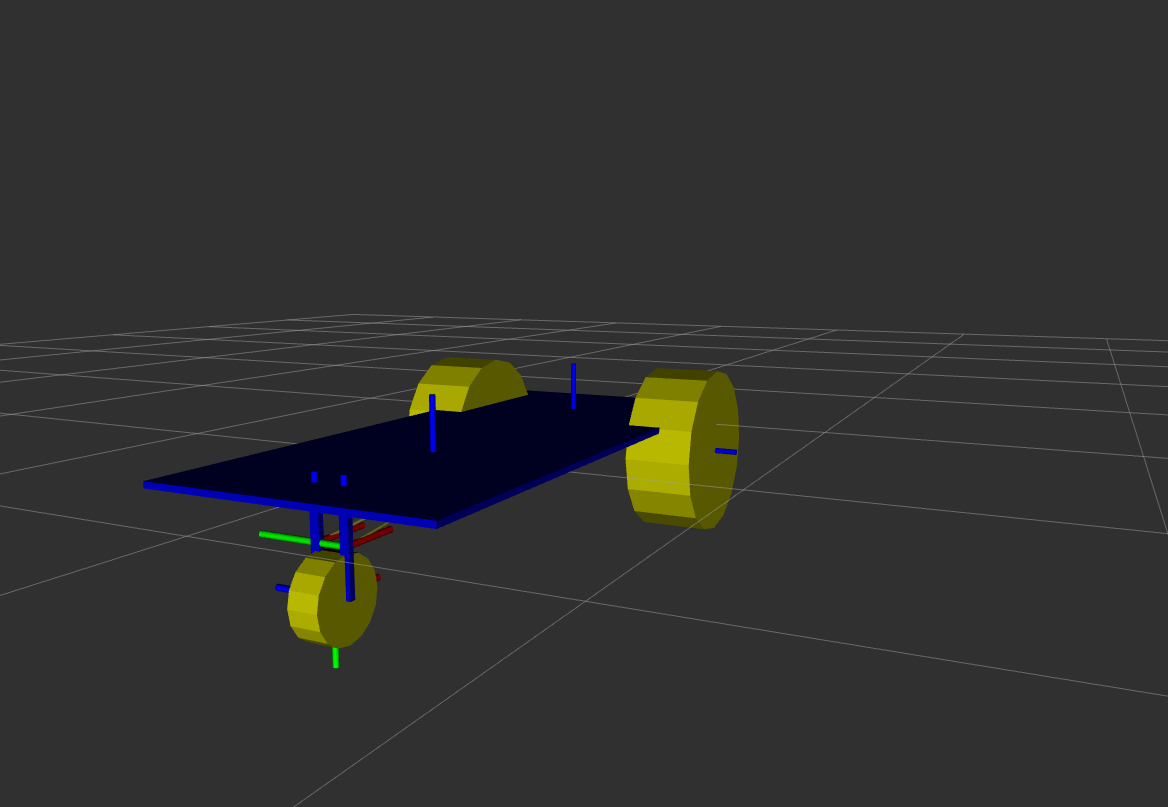
\includegraphics[width=0.7\textwidth]{Figures/fir_side.png}
    \caption{Primary Model}
    \label{fig:primary_model}
\end{figure}

\begin{figure}[h]
    \centering
    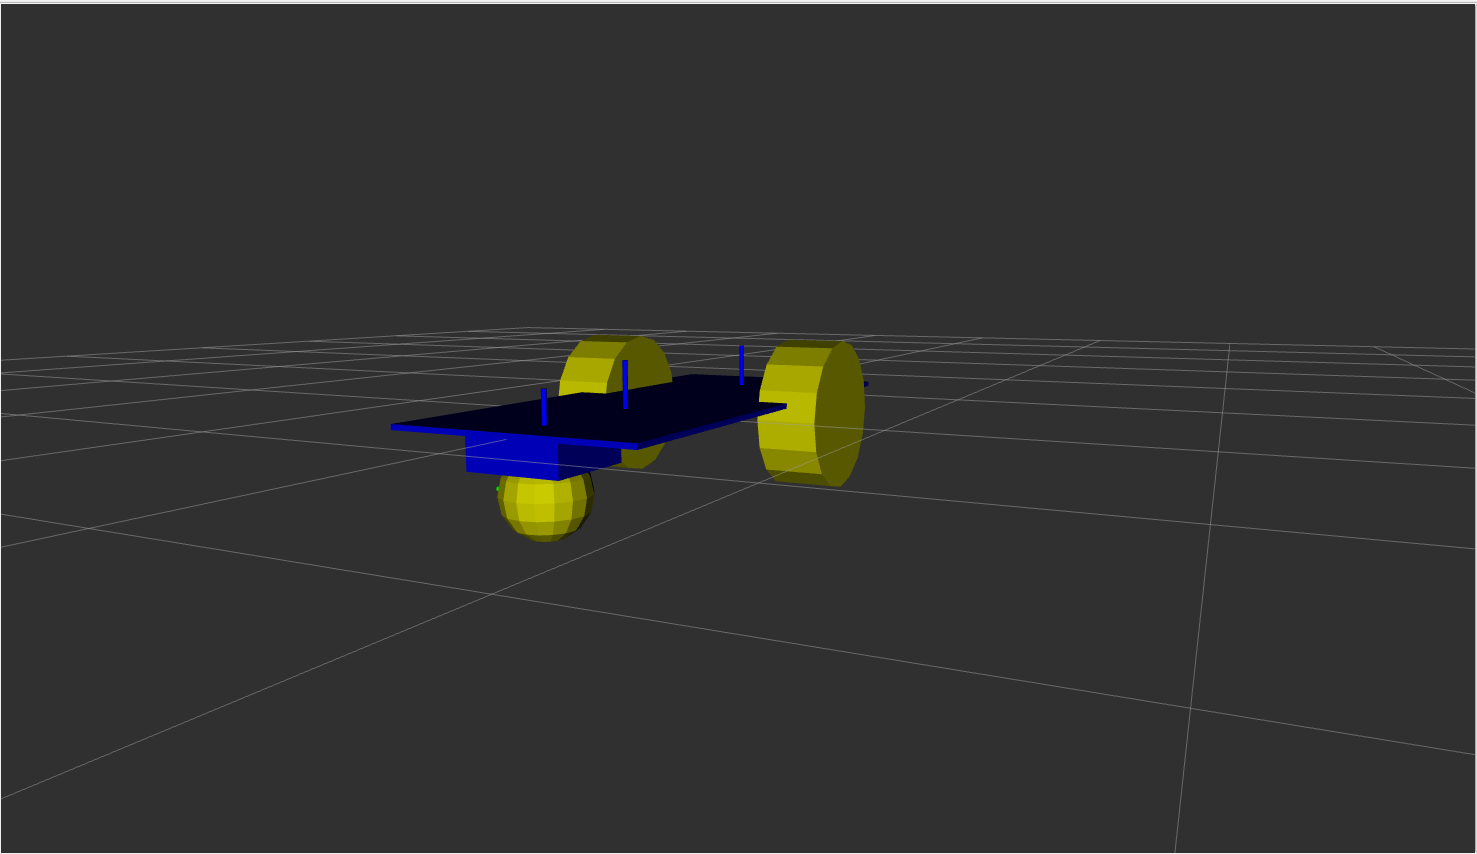
\includegraphics[width=0.7\textwidth]{Figures/sec_side.png}
    \caption{Second Model}
    \label{fig:second_model}
\end{figure}

\clearpage

In the final model, the additional link \verb|dummy_link| is added to generate a world-like layer. The idea is to vizualize a world component which could be used as a fix point on which the model could be placed and move around. This idea is then implemented, with in the gazebo simulation, but not further followed for the Rviz2 model. The final tf2 tree structure is shown in the figure~\ref{fig:tf_tree}.

\begin{figure}
    \centering
    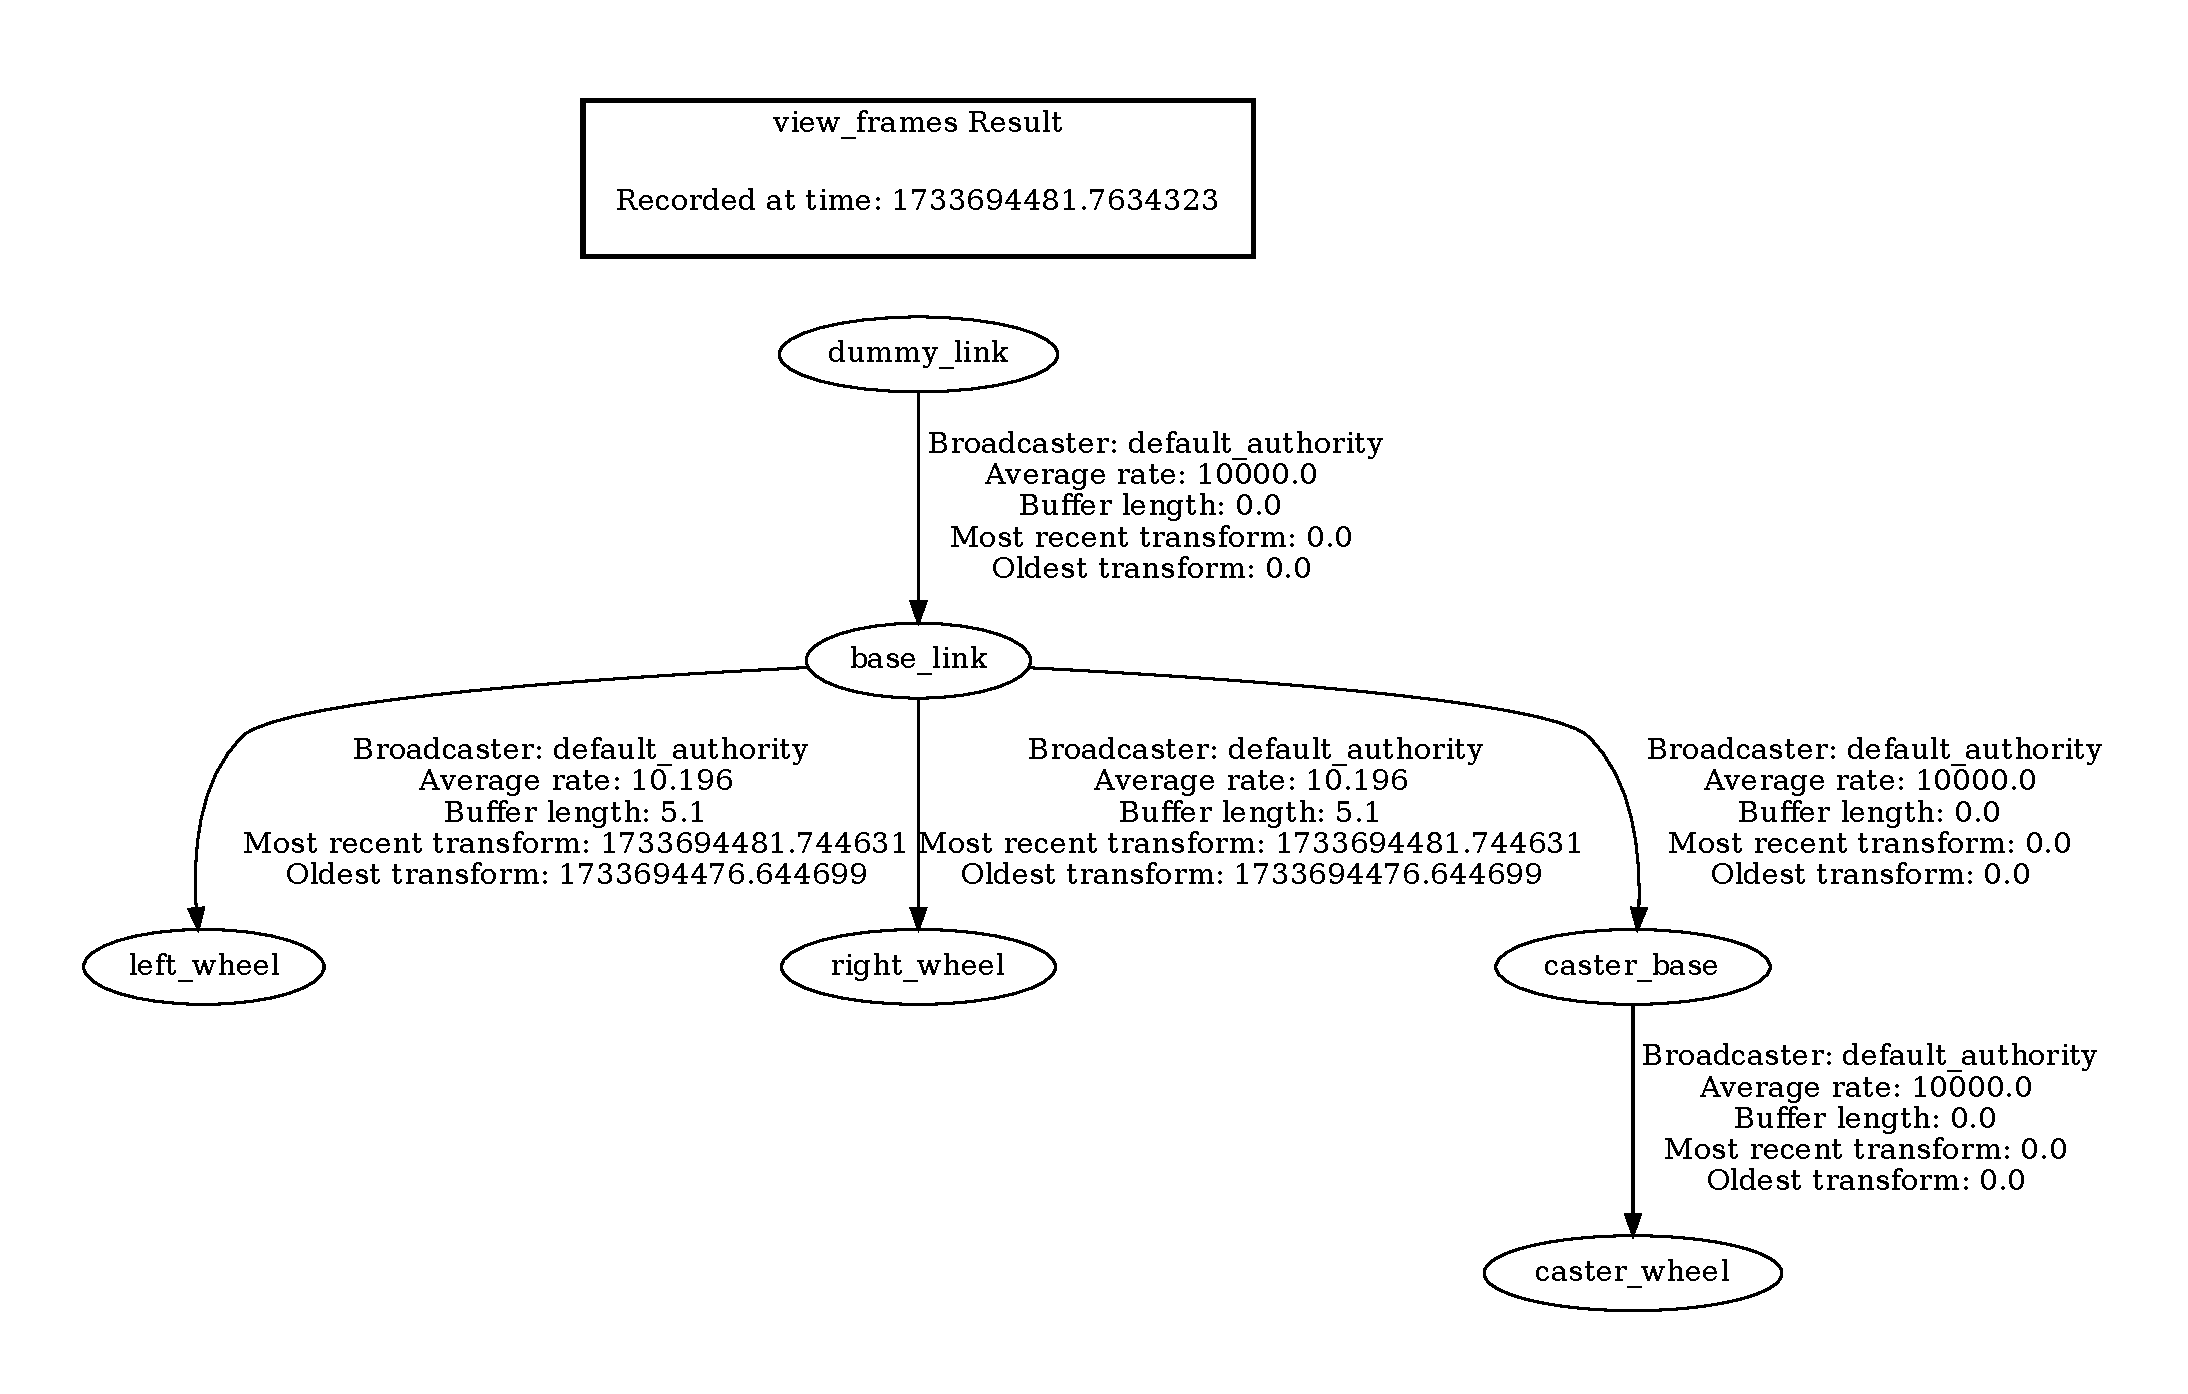
\includegraphics[width=0.7\textwidth]{Figures/frames_2024-12-08_22.48.01.pdf}
    \caption{tf2 tree structure}
    \label{fig:tf_tree}

\end{figure}

\begin{figure}
    \centering
    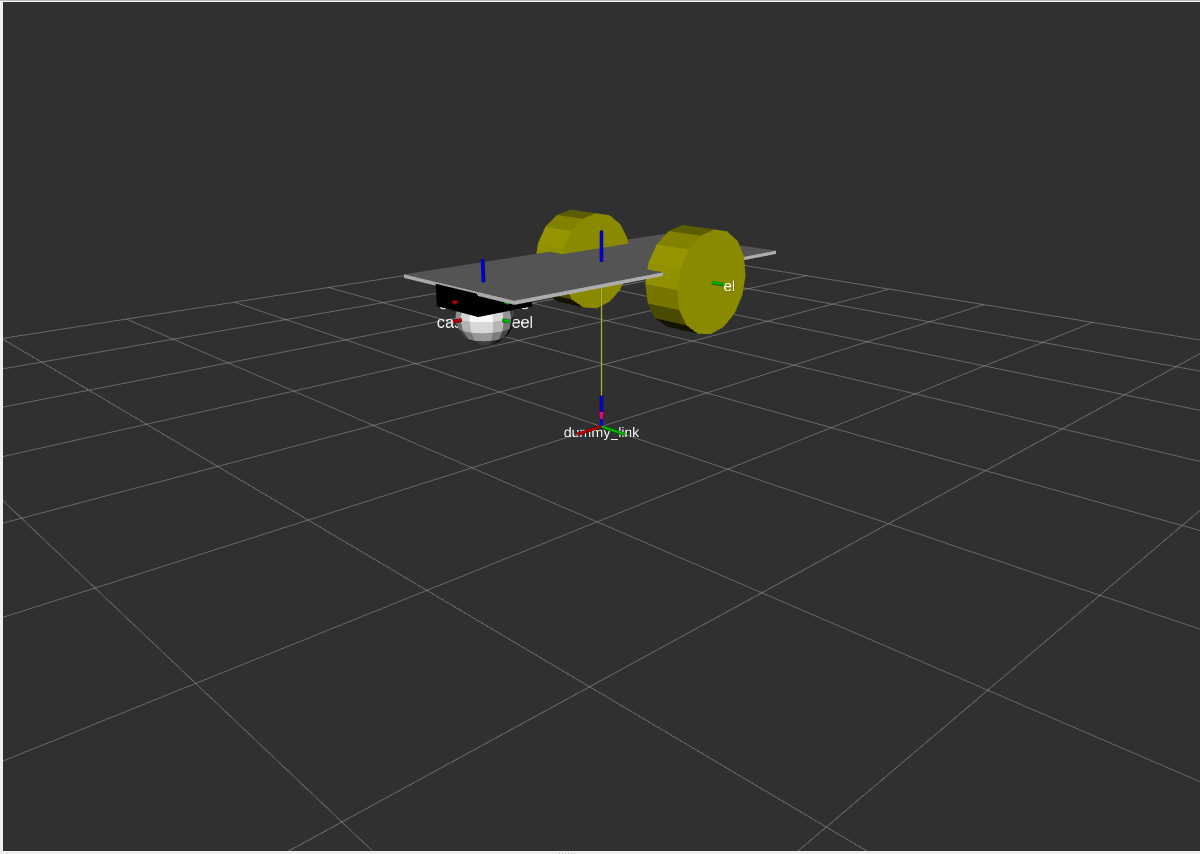
\includegraphics[width=0.7\textwidth]{Figures/final_model.png}
    \caption{Final Model}

\end{figure}


\clearpage

\section{Gazebo}

%% CG: No past tense! Please state how you installed GAZEBO and what you found out for choosing the correct version!
%% THis paragraph is missing references. 
The Gazebo simulator is successfully installed and launched. However, initial attempts to use the simulator fail due to the installation of an outdated version. The simulator is initially installed using the default method, which installs Gazebo Harmonic. Since compatibility between the ROS2 distribution and the Gazebo version is critical, Gazebo Ionic is installed to resolve the issue. The detailed installation prozess can be faund in the installation guide A3. 
Early attempts to integrate the Gazebo plugin into the URDF file were unsuccessful, as the necessary knowledge to perform this task is not yet acquired at this stage of the project. 
%% CG: SDF is not mentioned earlier. What provides the SDF file that goes beyond URDF?
To address this, the URDF file is converted into an SDF file. This translation allowed the model to be launched successfully in the simulator. The conversion process involved starting an empty world, a default package provided by Gazebo, and placing the URDF model into it. The robot is then successfully positioned on the floor within the simulation. Within the SDF file, the DiffDrive plugin is integrated, enabling the movement of the simulated robot. Forward and backward motion worked seamlessly; however, turning left and right posed challenges. 

%% CG: Better: Connecting the gazebo model to ROS2 failed on multiple occasions.
%% But why?
Also, the attempt to create a connection between the gazebo model and 
%% CG: ROS2 or ROS2? please be consistent.
ROS2 failed on multiple occasions, due to the wrong implementation of the \verb|gz_ros_bridge| node.
%% CG: This is resolved by ...
To solve this problem the ROS2 control and ROS2 controller packages could have been used, these packages are widely used in the ros community and offer a variety of control protocols and demonstration models, which show how to implement the packages, in the process of building a control system for the model and real-world robot. Multiple attempts were made to implement the packages and use them to control the model in the gazebo simulation, which all failed. Due to the time restrictions on this project, the attempt to work with this package is postponed to a further project.  In the final URDF file, the velocity and dynamics of the model were defined in more detail, and the gz\_controll.xacro which contains the differential drive plugin allowed the integration of the gazebo node in the launch file. The final model which is shown in the figure~\ref{fig:gazebo} could be moved seamlessly in all directions and could be controlled by sending messages to the /cmd\_vel topic.   

\begin{figure}[h]
    \centering
    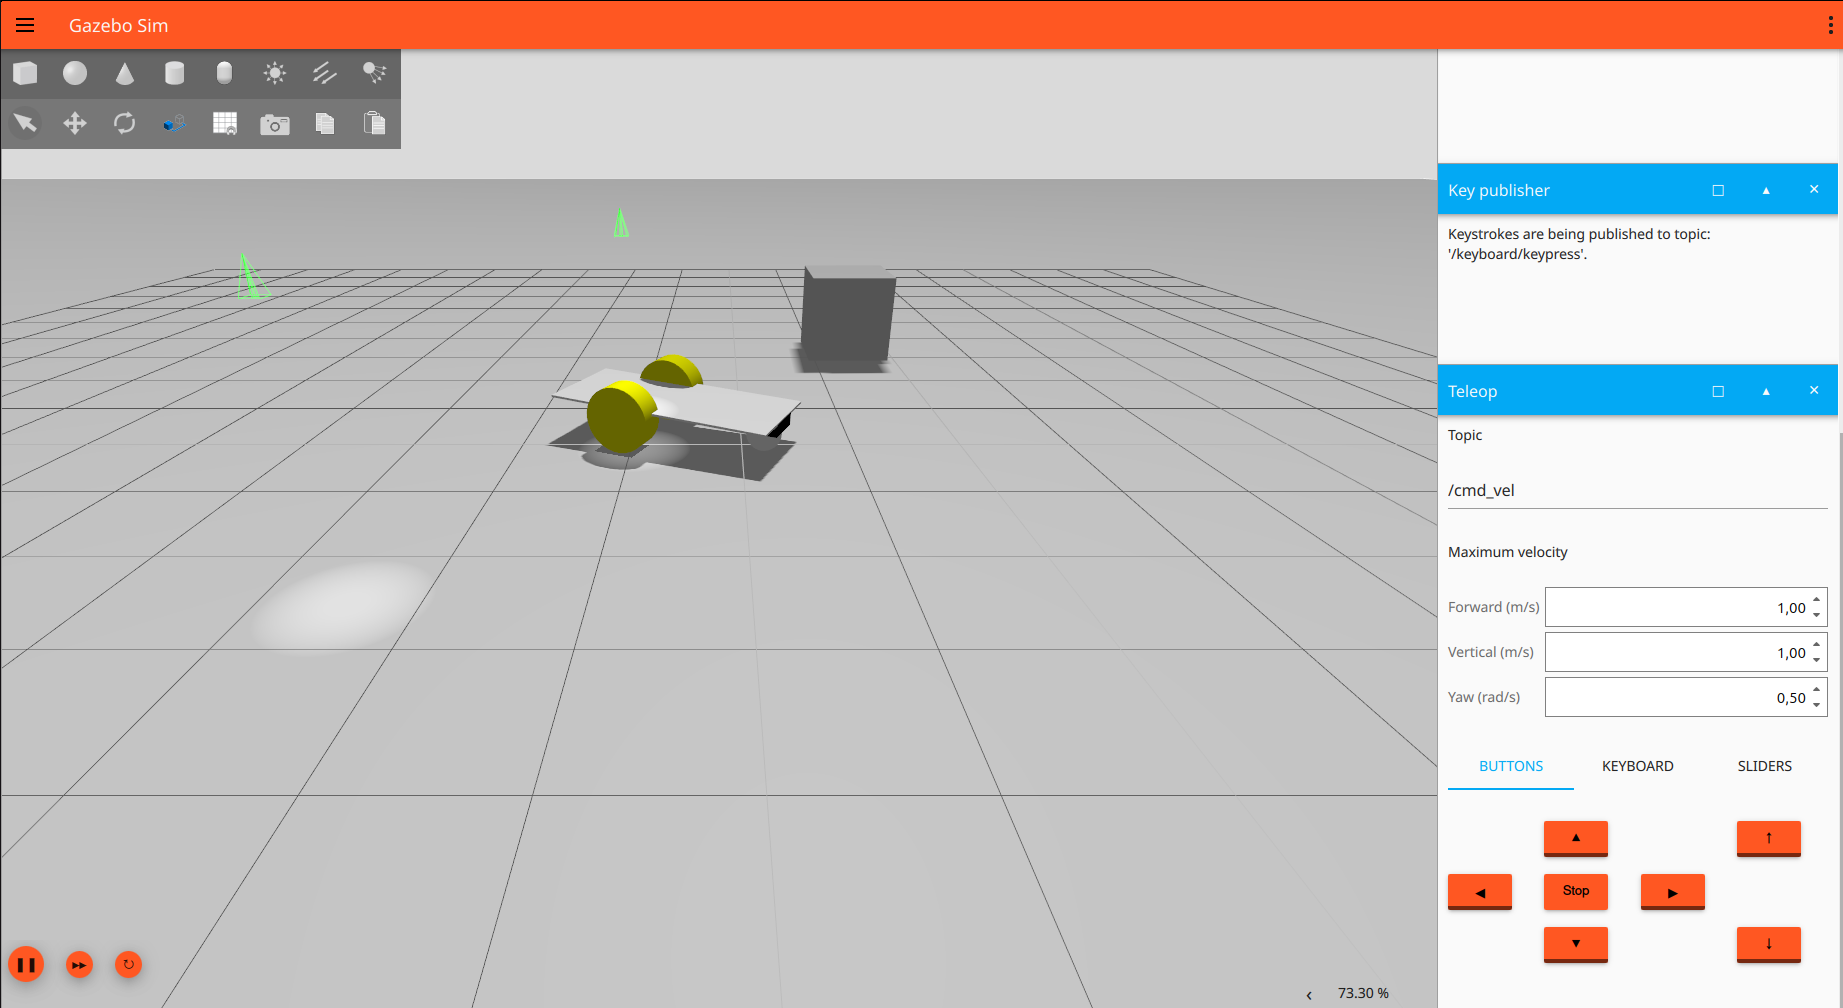
\includegraphics[width=0.7\textwidth]{Figures/gazebo_simulation.png}
    \caption{Gazebo Simulation}
    \label{fig:gazebo}

\end{figure}

\subsection{Controlling the real robot}

The primary remote control system for the real\-world robot is developed using two repositories the ros\_arduino\_bridge and serial\_motor\_demo. The serial\_motor\_demo provided two nodes and accompanying test scripts. The ros\_arduino\_bridge provided the Arduino scripts. Given that the project's requirements closely aligned with the two repository's existing components, it is possible to utilize the repositories for initial test runs with minimal code modifications. This approach significantly reduced development time within the project.
To enable customization without encountering permission conflicts, the repositories were first forked, creating an independent copy. These forked repositories were then cloned onto the control unit, the robot controller. To streamline the process of uploading scripts to the Arduino, the Arduino IDE is installed on the Raspberry Pi 4. A secure SSH connection between the laptop and the Raspberry Pi is established using Visual Studio Code's Remote extension. Additionally, the Arduino extension is installed in the remote environment, facilitating direct script uploads from the Raspberry Pi to the Arduino. The drive node is uploaded from the Raspberry Pi to the Arduino. The initial attempt to control the robot using the provided code is successful, representing a significant milestone in the project's progression.

\section{Building the digital twin}

At this phase of the project, the model could be visualised in Rviz2 and the wheel joints could be moved by using the joint state publisher. The model could be simulated with gazebo and controlled with the differential driver plugin. The real robot's movement could be enhanced by the ROS2 node gui.py and driver.py. The wheels could be moved separately and the speed could be adjusted.

In the first attempt to combine the elements, the ROS2 node \verb|gui.py| is altered. An attempt is made to connect the joint state publisher node with the \verb|gui.py| node. Therefore a message from the gui.py node is sent to the \verb|/joint_state| topic, where the message should be further passed to the joint state publisher node. This resulted in the movement of the wheel joints in the Rviz2 model. However, the model itself remained static. This could be explained by the lack of the dynamic implementation for the 
%% CG: Inconsistent capitalisation (see method section)
Rviz2 model. 

A further attempt is made by including the ``odom'' node. The odometry system %% CG: REFERENCE!
provides a locally accurate estimate of a robot's pose and velocity based on its motion. The odometry information can be obtained from various sources among other things the wheel encoders \autocite{SettingOdometryNav2}. Since the real robot did not include motor encoders a possible solution could have been to use the data representing the encoders of the digital twin. 


%% CG: It would help to have a visualisation of how the different components are connected.

This attempt is not further investigated, due to the time restrictions and complexity. Since the model staticity could not be overcome within the rivz2 environment the correct implementation of the tool is postponed to the following project. The further development of the digital twin is established in Gazebo. The \verb|gz_ros_bright| node is used to establish a connection between ROS2 and Gazebo. The gui.py node is exchanged with a \verb|self-developed| node. The \verb|cmd_vel_to_motor_command| node translates the speed values from the \verb|/cmd_vel| topic in a format which the motor controller could process. The two messages were sent simultaneously to the model and the real-world robot. The node functions as the interface between the robot and the gazebo simulation. By operating the control panel or sending commands over the terminal the model and the robot could be moved synchronously.



% Chapter 4: Discussion
\chapter{Discussion}

\section{Achievements}

The primary objective of the project, to develop a DT for an autonomous robot, was achieved, albeit with adjustments to the complexity of the digital twin. Throughout the project, a functional URDF file could be developed along with the \verb|cmd_vel_to_motor_command| node. The URDF file could be spawned in the visualization tool rviz2 and the simulator gazebo.  
%% CG: the launch file is needed for starting the sumulation and visualization tools ...
A launch file could be developed which started the simulation and visualization tools, along with the necessary nodes to display and control the model. 
Two motors are the actuators of this project. They are simulated by the differential driver plugin that provides basic movement functionality for the digital twin.  
Further, the connection between the control unit and the edge device could be established and motor speed commands could be sent and received from the control unit to the edge device. The simulator gazebo and ros2 could communicate over the \verb|gz_ros_bright| enabling the \verb|cmd_vel_to_motor_command| node to send and receive messages from the \verb|cmd_vel_to_motor_command| topics. 

\section{Functionality and Limitations}

While the simulation replicated the robot's movement, \verb|real-time| synchronization was not achieved. Furthermore, the digital twin was a simplified representation of the robot, lacking the integration of sensors and environmental elements. The \verb|/cmd_vel| and \verb|motor_command| node facilitated the sending of a command to the motor controller but did not allow the motor controller to transmit feedback messages, such as actual speed or encoder data. In a sophisticated system, the motor controller should be able to send feedback messages. By doing so a node like the odometry node could compare the velocity and speed data of the real-world robot and the digital twin. This comparison is essential for real-time synchronization. However, due to the unsuccessful implementation of the Odom node, the model does not receive feedback messages from the real robot, limiting the ability to perform bidirectional communication and validation. Consequently, the digital twin serves more as a reflection of the robot's state rather than a true twin with bidirectional feedback. 
The present model does not include any sensors as they increase the complexity of the robot significantly. This complexity is needed to meet the final objective but is beyond the scope of this project.


\subsection{Challenges and Bottlenecks}

The installation phase of this project provided a valuable learning experience as well as one of the main challenges. It involved exploring several methods for installing ROS2 to identify the most suitable approach for the project. This phase was particularly valuable, as it showed the benefits and limitations of different environments and installation techniques.
Several environments were tested, including VirtualBox, WSL2, Docker, and Ubuntu 24.04 Linux. While these were the primary tools explored for this step, the testing process allowed for a deeper understanding of how each method operates and interacts with ROS2's ecosystem.
This testing phase required significantly more time than initially anticipated, but it deepend the understanding of each environment.
Additionally, the understanding of the complex ecosystem of ros2 required substantial effort, making it one of the most time\-consuming aspects of the project. One of the challenges regarding the understanding of the ros2 systematics was the installation of 
%% CG: use compontents instead of tools. 
%% A tool is something that you use alongside of ROS, a component is part of the ROS environment.
additional components. 
These installations often failed due to version conflicts within the components and packages used. This problem was primarily caused by the choice of a developer distribution instead of a LTS version. The developer distribution is better suited for projects requiring cutting\-edge packages or tools not yet part of the LTS version and for developers with substantial experience in the ROS 2 ecosystem. Neither of these conditions was applicable in this project, making the developer distribution an unsuitable choice. The choice of the developer distribution is likely to have contributed to the unsuccessful implementation of ros2\_control and ros2\_controller. However, this remains uncertain, as other factors, such as limited familiarity with the ros2 ecosystem or configuration complexities, may also have played a role. Further, the time point of the establishment of a connection between the control unit and the edge device was later achieved as anticipated. This caused the project to stagnate. 


% Chapter 5: conclusion
\chapter{Conclusion and outlook}

\section{Conclusion}

Overall, the project achieved its fundamental objective but in a simplified form. The digital twin successfully mirrors the robot's behaviour to a degree but lacks real-time synchronization, environmental representation, and sensor integration. Within the project, a primary attempt was made to use the ros2 ecosystem to generate a digital twin. A deeper understanding of the ros2 applications could be established up to an extent, where a functional ros2 node could be developed and the native ros2 communication system could be used to control a real-world robot and a gazebo model. The choice of distribution and installation challenges significantly impacted the project's progress and complexity, but provided a deeper understanding of the configuration within the ros2 ecosystem.

\section{Outlook}

%% CG: maybe use "cornerstone" instead of "foundation"

%% CG: if it is your bachelor thesis, you should use the personal pronoun "my" instead of "a".

This project served as the cornerstone for a bachelor thesis, which aims to develop an autonomous robot tailored for the envisioned application of maintaining green rooftop ecosystems with photovoltaic panels installed.
Key advancements to be addressed based on the project presented, include the integration of feedback mechanisms from the motor controller. This addition would enable data-driven comparisons between the digital model and the physical robot, enhancing precision in control and orientation. Furthermore, the simulation environment should be refined to accurately represent the rooftop green spaces where the robot will operate. For this detailed simulation, an alternative to Gazebo could be a more efficient solution since the gazebo simulator's complexity rises with the complexity of the model. Implementing sensors such as cameras, infrared systems, or lasers would be critical to ensure the robot can effectively perform its tasks. The implementation of neural networks and advanced algorithms would be essential for the development of a robust object detection and decision-making system. To streamline the development process and enhance deployment flexibility, using Docker containers for the ROS2 system would ensure portability, consistency, and simplified setup while enabling efficient cross-device deployment and resource isolation. Finally, the robot design of the presented project would not meet the functional requirements for maintaining rooftop ecosystems. Therefore, a new robot design is be needed that would include a new URDF file for the digital twin.


%----------------------------------------------------------------------------------------
% BIBLIOGRAPHY
%----------------------------------------------------------------------------------------
\printbibliography[heading=bibintoc]
\clearpage
%----------------------------------------------------------------------------------------
%----------------------------------------------------------------------------------------
% THESIS CONTENT - APPENDICES
%----------------------------------------------------------------------------------------
\pagenumbering{gobble}
%\listoffigures
%\listoftables
\appendix % Cue to tell LaTeX that the following "chapters" are Appendices

% Include the appendices of the thesis as separate files from the Appendices folder
% Uncomment the lines as you write the Appendices

\chapter{Installation guides}

\label{Apendix1} % Change X to a consecutive letter; for referencing this appendix elsewhere, use \ref{AppendixX}

\section{Change Operating System of Control Unit}

\subsection{Objective}
To simplify the work experience, a change in the main operating system on the control unit was performed. The original OS was Windows 10, and the target OS was Ubuntu 24.04 LTS.

\subsection{Procedure}
To perform the reboot of the OS, the following steps were taken:

\subsection{Preparation: USB Stick and ISO Image}
\begin{itemize}
    \item USB Stick with 128GB.
    \item Download the Ubuntu ISO: \href{https://ubuntu.com/download}{https://ubuntu.com/download}.
\end{itemize}

\subsection{Step 1: Create a Bootable USB Stick (For Windows Users)}
Download and Start Rufus (on Windows)
\begin{itemize}
    \item Download Rufus: \href{https://rufus.ie/de/}{https://rufus.ie/de/}.
\end{itemize}

\subsubsection{Configure Rufus Settings}
\begin{itemize}
    \item \textbf{Device:} Select the USB stick in the “Device” dropdown menu.
    \item \textbf{Boot Selection:} Click “SELECT” and choose the Ubuntu ISO file downloaded earlier.
    \item \textbf{Partition Scheme:}
    \begin{itemize}
        \item Select \textbf{GPT} when using UEFI.
        \item Select \textbf{MBR} when using an older BIOS or UEFI with CSM (Compatibility Support Module).
    \end{itemize}
    \item \textbf{Target System:}
    \begin{itemize}
        \item UEFI (non-CSM) for newer devices.
        \item BIOS (or UEFI-CSM) for older devices.
    \end{itemize}
    \item \textbf{File System:} FAT32.
\end{itemize}

\subsubsection{Start the Process}
\begin{itemize}
    \item Wait for the process to complete.
\end{itemize}

\subsection{Step 2: Boot Ubuntu from the USB Stick}
\begin{itemize}
    \item Plug in the USB stick and restart your laptop.
    \item Open the Boot Menu:
    \begin{itemize}
        \item Use one of the following keys: F12, F10, Esc, or Del.
    \end{itemize}
    \item Select the USB stick as the boot device to start Ubuntu.
\end{itemize}

\subsection{Step 3: Install Ubuntu}
Start the Installation
\begin{itemize}
    \item Follow the installation guide.
\end{itemize}

Choose Installation Type
\begin{itemize}
    \item Example: \textbf{“Erase disk and install Ubuntu”} to remove Windows and use only Ubuntu.
\end{itemize}

Advanced Features (Optional)
\begin{itemize}
    \item Configure as needed.
\end{itemize}

Confirm Installation
\begin{itemize}
    \item Wait for the process to complete.
\end{itemize}

\subsection{Step 4: After Installation}
\begin{itemize}
    \item Remove the USB stick and restart.
    \item Use Ubuntu.
\end{itemize}

\clearpage
\section{Install ROS2 on Ubuntu 24.04}

\subsection{Objective}
The Objective of this experiment was to install ROS2 rolling, on the controll unit (Laptop HP with Ubuntu 24.04) and the Raspberry Pi (also with Ubuntu 24.04). 
The main issue was to creat a connention between the machines. 

\subsection{Procedure}
The first step was to install ROS2 rolling desktop on both machines. For that the instructions from the ros2 website where used. 
\url{https://docs.ros.org/en/rolling/Installation/Ubuntu-Install-Debs.html}

After the installation the source command for ROS2 setup file was added to the .bashrc file on both devices. 
\begin{lstlisting}[language=bash]
    #oben file via editor
    nano ~/.bashrc
    # add the command on the botton of the file
    source /opt/ros/rolling/setup.bash
\end{lstlisting}

To creat a connention between the machines the following steps were follwed, on both machines.
The ROS\_IP and the ROS\_DOMAIN\_ID where addet after the source command for the ros2 setup file, within the .bashrc file.
The ROS IP adresse represented the IP adresse of the current machine, and the ROS DOMAIN ID was the same domain number for both machines. 


\begin{lstlisting}[language=bash] 
    export ROS_DOMAIN_ID=0
    export ROS_IP=192.168.x.xx
    \end{lstlisting}

Then the .bashrc file was sourced on both machines with the following command:
\begin{lstlisting}[language=bash] 
    source ~/.bashrc
    \end{lstlisting}


    \subsection{Testing}
To test if the two machines could communicate a demo node of ROS2 was used. 
Therefore the two commands:
\begin{lstlisting}
    ros2 run demo_nodes_cpp talker
    ros2 run demo_nodes_py listener
\end{lstlisting}

Where used, one machine was sending a messeage with the talker, and the other reseved the message with the listener. 

\subsection{Additional}
If the connection still can't be astablished the following steps can be tryed:

1. Check if your SSH-Connection works correctly. 

2. Check your firewall status 

3. When using a virtuell machine, make sure your controll unit is connetet through etahl cable to the network, and not over wlan. 


\clearpage
\section{Install Gazebo Ionic}

\subsection{Objective}
The inidial try to install gazebo was by using the defalt installation. Therefore the command:
\begin{lstlisting}[language=bash]
    sudo apt install ros-rolling-ros-gz 
\end{lstlisting}

was used. This installed a version von gazebo which was to old for the ubunt 24.04 operation system. 
Due to this the error
\begin{lstlisting}[language=bash]
    [GUI] [Err] [Ogre2RenderEngine.cc:1301]  Unable to create the rendering window: 
    OGRE EXCEPTION(3:RenderingAPIException): currentGLContext was specified with no current GL context 
    in GLXWindow::create at ./.obj-x86_64-linux-gnu/gz_ogre_next_vendor-prefix/src/gz_ogre_next_vendor/RenderSystems/GL3Plus/src/windowing/GLX/OgreGLXWindow.cpp (line 165)
\end{lstlisting}
    

accuret. This leat to the interution of the simulation, before the simulation could be loaded the programm was killed. 

\subsection{Procedure}
As describet on the official website of gazebo, a specific version of gazebo had to be installed. For ROS2 Rolling the Gazebo Ionic was compartible. 
After removing the humble version of gazebo, the ionic version was installed by following the instructions of the official website: 

\begin{lstlisting}
    https://gazebosim.org/docs/latest/install_ubuntu/
\end{lstlisting}



\chapter{Use of AI Tools in the Project}
In this project, various AI tools were utilized. The specific tools and their roles are outlined below:

\section*{AI Tools}
\begin{itemize}
    \item \textbf{DeepL}: Used for translating text
    \item \textbf{Grammarly}: Assisted in correcting grammatical errors and improving the overall readability of the text.
    \item \textbf{ChatGPT}:
    \begin{itemize}
        \item Assisted in synonym searches
        \item Corrected grammar and clarity of written content.
        \item Improved the structure and flow of the text
        \item Provided explanations for LaTeX functions and structures to streamline the document creation process.
    \end{itemize}
    \item \textbf{ChatGPT and Codeium}: Supported coding tasks by:
    \begin{itemize}
        \item Improving existing code snippets and structures.
        \item Explaining complex C++ code scripts and structures for better understanding and implementation.
    \end{itemize}
\end{itemize}


% from https://www.zhaw.ch/en/lsfm/study/studiweb/master-ls/masters-thesis/
%\include{Appendices/AppendixB}
%\include{Appendices/AppendixC}
%% !TEX root = ../main.tex

%----------------------------------------------------------------------------------------
% APPENDIX: DECLARATION OF ORIGINALITY
%----------------------------------------------------------------------------------------

% Include the official "Plagiatserklärung" as a PDF

% Ensure that a TOC entry is create while suppressing the chapter header
\cleardoublepage
\phantomsection
\addtocounter{chapter}{1}
\addcontentsline{toc}{chapter}{\protect\numberline{\thechapter} Declaration of Originality}
% The above replaces this command (which creates a chapter header).
%\chapter{Declaration of Originality} % Main appendix title
\label{DeclarationOfOriginalityZHAW}

% Include a PDF (full page)

\includepdf[pages=-]{Appendices/plagiatserklaerung-master-eng.pdf}
 


\end{document}  
